\documentclass[12pt,twoside,letterpaper,titlepage]{report}

\usepackage{amssymb,amsmath}
\usepackage{mathspec}
\defaultfontfeatures{Ligatures=TeX,Scale=MatchLowercase}
\usepackage[margin=0.75in, top=1in]{geometry}
% fixltx2e has been merged into LaTeX2e proper
% see: https://latex-project.org/ltnews/ltnews22.pdf
% \usepackage{fixltx2e}
\usepackage{graphicx,grffile}
\makeatletter
\def\maxwidth{\ifdim\Gin@nat@width>\linewidth\linewidth\else\Gin@nat@width\fi}
\def\maxheight{\ifdim\Gin@nat@height>\textheight\textheight\else\Gin@nat@height\fi}
\makeatother
% Scale images if necessary, so that they will not overflow the page
% margins by default, and it is still possible to overwrite the defaults
% using explicit options in \includegraphics[width, height, ...]{}
\setkeys{Gin}{width=\maxwidth,height=\maxheight,keepaspectratio}
\usepackage[table,svgnames]{xcolor}
\usepackage{framed}
\usepackage{longtable,booktabs}
\usepackage{listings}
\usepackage{enumitem}
\PassOptionsToPackage{hyphens}{url}\usepackage[breaklinks=true]{hyperref}

% Background Color for Note/Admonition Boxes
\definecolor{shadecolor}{rgb}{0.9,0.9,0.9}

% Band the Color of Rows in Tables
% unfortunately, doesn't seem to work across the board. Turning off for now
%\rowcolors{1}{white}{lightgray!25!white}

\newenvironment{callout}{\begin{shaded*}\small}{\end{shaded*}}
\newcommand{\warning}[1]{\small{\textbf{\textcolor[rgb]{0.8,0.2,0.2}{#1}}}}

% Font Settings
%\setmainfont[]{Calibri}
%\setmonofont[Mapping=tex-ansi]{Inconsolata}
%\usepackage{newtxtext,newtxmath}

% The depth of numbering for sections
\setcounter{secnumdepth}{4}

% Listing Settings
\lstset{
  backgroundcolor=\color{BlanchedAlmond!20!white},
  basicstyle=\ttfamily\scriptsize,
  breakatwhitespace=false,
  breaklines=true,
  frame=bottomline,
  keepspaces=true,
}

% Provide better table spacing
% From https://www.inf.ethz.ch/personal/markusp/teaching/guides/guide-tables.pdf
\renewcommand{\arraystretch}{1.2} 

\graphicspath{{media/}}

\pagestyle{headings}

% Define custom commands from Pandoc
\setlength{\emergencystretch}{3em}  % prevent overfull lines
\providecommand{\tightlist}{%
  \setlength{\itemsep}{0pt}\setlength{\parskip}{0pt}}

% Redefine (sub)paragraphs to behave more like sections
\ifx\paragraph\undefined\else
\let\oldparagraph\paragraph
\renewcommand{\paragraph}[1]{\oldparagraph{#1}\mbox{}}
\fi
\ifx\subparagraph\undefined\else
\let\oldsubparagraph\subparagraph
\renewcommand{\subparagraph}[1]{\oldsubparagraph{#1}\mbox{}}
\fi

% this is a great package for printing units in a standard way, we should move this way
\usepackage{siunitx}

% some additional macros
\newcommand{\PB}[1]{\left(#1\right)}
\newcommand{\RB}[1]{\left[#1\right]}
\newcommand{\CB}[1]{\left\{#1\right\}}

\author{U.S. Department of Energy}
\date{September 30, 2016}


\title{Tips and Tricks for Using EnergyPlus}

\hypersetup{unicode=true,
            pdftitle={Tips and Tricks for Using EnergyPlus},
            pdfauthor={U.S. Department of Energy},
            colorlinks=true,
            linkcolor=Maroon,
            citecolor=Blue,
            urlcolor=Blue,
            breaklinks=true}
\urlstyle{same}  % don't use monospace font for urls

\begin{document}


\input{../title}


\chapter{Introduction \& Support}\label{introduction-support}

This is a quick guide for using and troubleshooting EnergyPlus simulation software. The information here is taken from the knowledge base and from EnergyPlus users looking for answers.

\textbf{Note that these articles are taken from actual user questions and may not be applicable to your model.}

For more detailed information about using EnergyPlus, refer to the user guides and manuals that are installed in the Documentation folder and are also available from \href{https://energyplus.net}{www.energyplus.net}.

This is a short guide

\ldots{} meant to save time and energy!


\section{Organization}\label{organization}

The organization of this document roughly uses the categories of the new features documents that have been included with EnergyPlus since April 2001 (the initial offering).

Under the subject categories, there may be a mix of short articles and Q\&A format.


\section{EnergyPlus Support}\label{energyplus-support}

\textbf{Please refer to the Support page for up to date information}: \url{https://energyplus.net/support}

The primary EnergyPlus support site is supplied at: \url{https://energyplushelp.freshdesk.com/}

The site is monitored by EnergyPlus developers and questions are attempted to be answered in a timely manner. Standard EnergyPlus support is provided free of charge by the U.S. Deparment of Energy, as part of a continuing effort to improve the EnergyPlus building simulation tool. Expedited, priority support may be available from other sources. The helpdesk has a files area where important (after release) files may be put as well as the storage for the Transition file set that are prior to the current release.


\section{General}\label{general}

\subsection{Schedules}\label{schedules}

A series of actuators is available for overriding schedule values. The following actuators are available with the control type called ``Schedule Value'':~ Schedule:Year, Schedule:Compact, Schedule:File, and Schedule:Constant. The units are not known by the schedule and are determined by the model that references the schedule. The unique identifier is the name of schedule.

If you try to use a particular schedule as input to calculations that modify that schedule, you will be in a circular situation with unexpected results. The modified schedule will lose the original information (unless the actuator is set to Null) and the modifications will be reapplied on top of previous modifications. When this situation arises, use a copy of the original schedule as input to the Erl program so you have the original schedule values.

\subsection{Curves}\label{curves}

An advanced actuator called ``Curve'' with a control type called ``Curve Result'' is available whenever any generic curve objects are used. This allows you to override the results generated by these curves. The units are not known by the actuator and depend on how the curve is being used by the component model that calls it.

This actuator must be used with caution. The EMS does not necessarily have access to the independent variables used by the models when the curves are evaluated during normal evaluation, so in most situations you will probably need to examine EnergyPlus source code to use this actuator correctly.

\subsection{Weather Data}\label{weather-data}

A series of actuators called ``Weather Data'' are available for overriding the values of weather data that are normally derived from the .epw weather file. These provide the ability to alter weather data and were originally requested for use with ExternalInterface for using measured data. The unique identifier is ``Environment''. The following can be overridden, using these names for the Actuated Component Control Type: Outdoor Dry Bulb, Outdoor Dew Point, Outdoor Relative Humidity, Diffuse Solar, Direct Solar, Wind Speed, and Wind Direction. EMS calling point BeginZoneTimestepBeforeSetCurrentWeather is the only EMS calling point called near the beginning of the zone timestep prior to ``SetCurrentWeather'' which is where these actuators are applied. Note that this calling point is not active during sizing.


\section{What EnergyPlus Is}\label{what-energyplus-is}

The primary website for EnergyPlus is \url{https://energyplus.net}

EnergyPlus is an energy analysis and thermal load simulation program. Based on a user's description of a building from the perspective of the building's physical make-up, associated mechanical systems, etc., EnergyPlus will calculate the heating and cooling loads necessary to maintain thermal control set points, conditions throughout a secondary HVAC system and coil loads, and the energy consumption of primary plant equipment as well as many other simulation details that are necessary to verify that the simulation is performing as the actual building would. More details on what EnergyPlus is can be found in the \emph{GettingStarted Document}.

No program is able to handle every simulation situation. However, it is the intent of EnergyPlus to handle as many building and HVAC design options either directly or indirectly through links to other programs in order to calculate thermal loads and/or energy consumption on for a design day or an extended period of time (up to, including, and beyond a year).


\section{What EnergyPlus Isn't}\label{what-energyplus-isnt}

\begin{itemize}
\tightlist
\item
  a user interface. It is intended to be the simulation engine around which a third-party interface can be wrapped. Inputs and outputs are simple ASCII text that is decipherable but may be best left to a GUI (graphical user interface). The current known third-party interfaces/tools can be found at
\end{itemize}

http://apps1.eere.energy.gov/buildings/energyplus/interfaces\_tools.cfm

\begin{itemize}
\item
  a life cycle cost analysis tool. It produces results that can then be fed into an LCC program.
\item
  an architect or design engineer replacement. It does not check input, verify the acceptability or range of various parameters (expect for a limited number of very basic checks), or attempt to interpret the results. However, it does have several reporting features to help you do exactly that.
\end{itemize}


\section{Getting Started}\label{getting-started}

If you're familiar with building simulation, use the 300+ example files that come with the program and the Input/Output Reference to help you.

If you're new to building simulation, read and work through the tutorials in the ``Getting Started'' document or visit the online tutorial, \url{http://www.vibyor.com} (tutorial was created by Prof.~Vishal Garg from IIIT Hyberabad, India).

Another avenue you might use is the EnergyPlus Example File Generator (EEFG) program, which will not only produce an input file for your later use, but also run your specifications on EnergyPlus and send you the results. EEFG is available through the interface page referenced above or \url{http://apps1.eere.energy.gov/buildings/energyplus/cfm/inputs/}.


\section{Comparing EnergyPlus to Other Programs}\label{comparing-energyplus-to-other-programs}

A paper comparing and contrasting Energy Simulation Programs can be found here:

\url{http://www.eere.energy.gov/buildings/tools_directory/pdfs/contrasting_the_capabilities_of_building_energy_performance_simulation_programs_v1.0.pdf}

As this paper was published in 2005, it is out of date (at least with current EnergyPlus capabilities).

The feature highlights from EnergyPlus releases can be seen here:

\url{http://apps1.eere.energy.gov/buildings/energyplus/pdfs/featurehighlights.pdf}

In addition you can see how EnergyPlus compares to other programs (which have submitted their models) in our testing reports:

\url{http://apps1.eere.energy.gov/buildings/energyplus/testing.cfm}


\section{DataSets}\label{datasets}

Akin to the libraries of other programs, EnergyPlus uses data sets.~ Data sets are similar to libraries but many items are contained in a single file (usually input file format or sometimes macro format).~ Developers are encouraged, as appropriate, to submit data sets along with new features.~ Some of the existing data sets include:

\begin{itemize}
\item
  Materials properties
\item
  Construction elements (layers of materials)
\item
  Composite construction definitions (equivalent constructions for complex elements)
\item
  Solar Collector parameters
\item
  Economic Tariffs
\item
  Design Day definitions
\item
  Location definitions
\item
  Standard report definitions
\end{itemize}


\section{Datasets aka Libraries}\label{datasets-aka-libraries}

EnergyPlus uses the term DataSets for what many would call libraries. These files are included, for the most part, in the instalation package but may be available from other sites (such as the helpdesk or Yahoo Groups).

There are two flavors of DataSets: \textbf{simple} and \textbf{Macro}. Some sets have files in both camps (for example, Solar Collectors). Both flavors contain IDF objects ready to be put into EnergyPlus input files. With the simple datasets, you may need to use a text editor or the IDF Editor to search the file for the one you want to use.~ With the macro datsets and a simply structured imf (input macro file), you can name the item you want to include. (The macro program is described in the \href{file:///E:/Docs4PDFs/AuxiliaryPrograms.pdf}{Auxiliary Programs document}).

Primary documentation for each dataset is found in the \href{file:///E:/Docs4PDFs/OutputDetailsAndExamples.pdf}{Output Details and Examples document}. Highlights of some datasets are given here.


\section{Locations-DesignDays}\label{locations-designdays}

This file (Locations-DesignDays.xls) can be found in the MacroDataSets folder. While not strictly a macro file, it leads one to be able to download the ASHRAE design day definitions from the EnergyPlus website. The spreadsheet format contains a sheet for each of the WMO regions as well as the California Climate Zones, specifically sheets included are:

\begin{itemize}
\item
  Readme -- an upfront readme page
\item
  WMO1 Africa
\item
  WMO2 Asia
\item
  WMO3 South America
\item
  WMO4 North \& Central America
\item
  CZ Files -- California Climate Zones
\item
  WMO5 Southwest Pacific
\item
  WMO6 Europe
\item
  WMO7 Antarctica
\end{itemize}

Each WMO (World Meteorological Organization) page contains the countries represented, specific cities that have design conditions data from ASHRAE, a link to the full imf file with location, daylighting saving and design day definitions as well as a link to that region's weather page on the EnergyPlus website. Pressing the links here will allow you to download the files.


\chapter{Design Day / Weather Data}\label{design-day-weather-data}


\section{Design Day Creation}\label{design-day-creation}

\emph{How do I create the profile used in the SizingPeriod:DesignDay object?}

Typically, the EnergyPlus Development Team uses the data from the most recent ASHRAE Handbook of Fundamentals to create a set of design day profiles that can be used. Description of ASHRAE's data is contained in Chapter 14 of the 2009 Handbook of Fundamentals. Table~\ref{table:multistory-vs-multistory-2-and-multistory-3} shows the kind of data that is embodied in the design day definitions shown earlier (ref. Locations-DesignDays).

Design Days (aka Design Conditions) are very important for use in HVAC Sizing calculations -- refer to the ASHRAE Handbook of Fundamentals for further information.

From this, you can determine if you should use one of these profiles and modify it or determine how to create your own profile.

The Weather Converter program accesses this file when it processes (even for statistics) a weather file. Design Day definitions are also included with the zips on the EnergyPlus weather data site. For locations that don't have ASHRAE design conditions, the Weather Converter uses the data within the weather file to generate pseudo conditions in the statistics file.


\section{EPW Weather Files}\label{epw-weather-files}

The WeatherConverter converts from other source formats to EPW and EnergyPlus CSV formats. The WeatherConverter also produces a statistics file that provides a quick synopsis of the converted data and is used by the tabular reports (ref: Climatic Data Summary report). For Ecotect users, the Weather Converter can also save as .wea format. We do not support conversion of EPWs to other formats, including to TMY2. The Weather Converter is described in detail in the \href{file:///E:/Docs4PDFs/AuxiliaryPrograms.pdf}{Auxiliary Programs document}.


\section{Meteonorm Weather Files}\label{meteonorm-weather-files}

For locations that aren't on the regular EnergyPlus weather site (\url{https://energyplus.net/weather}), the team has created weather data using the Meteonorm\textsuperscript{TM} software.
Meteonorm extrapolates hourly data from statistical data for a location. Where statistical data aren't available, Meteonorm interpolates from other nearby sites.
Generally, a statistical approach is a last resort---weather files generated from statistics will not demonstrate the normal hour-to-hour and day-to-day variability seen in measured data.
Each .ZIP includes a .STAT (EnergyPlus weather data statistics), .EPW (EnergyPlus weather file), and .INFO (Information about the source data and limitations from Meteonorm).

In all cases, review the .STAT file for the location before using any of these files to ensure that it represents the climate of the locations as you understand it.
In many cases, a nearby location with measured data may be more appropriate than one derived from statistics.
These files, once created, are published on the EnergyPlus Yahoo Group site.

As always, if you know of sources of weather data that we might be able to share with the EnergyPlus community, please contact us.


\section{Weather Data for Simulations}\label{weather-data-for-simulations}

Weather data can be used for various purposes by simulation program such as EnergyPlus. For some purposes, such as validating a model to actual energy use, you may wish to match the weather data to the simulation period. However, for most purposes, you will wish to have a more typical weather data profile. Information on selecting weather data is described in this paper:

Drury B. Crawley. 1998. ``Which Weather Data Should You Use for Energy Simulations of Commercial Buildings?'' in ASHRAE Transactions, pp.~498-515, Vol. 104, Pt. 2. Atlanta: ASHRAE. (PDF 197 KB)

PDF: \url{http://energyplus.gov/pdfs/bibliography/whichweatherdatashouldyouuseforenergysimulations.pdf}


\section{Weather File Sources}\label{weather-file-sources}

The description of sources for the EnergyPlus weather data that is on the website are available here: \url{http://apps1.eere.energy.gov/buildings/energyplus/weatherdata_sources.cfm}


\section{Measuring Solar Data}\label{measuring-solar-data}

\emph{Can the following weather file metrics be directly measured by some inexpensive devices?}

Extraterrestrial Horizontal Radiation \{Wh/m2\} Extraterrestrial Direct Normal Radiation \{Wh/m2\} Horizontal Infrared Radiation Intensity from Sky \{Wh/m2\} Global Horizontal Radiation \{Wh/m2\} Direct Normal Radiation \{Wh/m2\} Diffuse Horizontal Radiation \{Wh/m2\} Global Horizontal Illuminance \{lux\} Direct Normal Illuminance \{lux\} Diffuse Horizontal Illuminance \{lux\}*

You can't measure extraterrestrial unless you're in outer space, but then it's assumed to be constant anyway. For the various radiation and illuminance values, they can measured by various instrumentation ranging from the very cheap to the very expensive. Properly, radiation needs to be measured with a pyranometer (Eppley), which is pricy, but I'm also seen people use simpler apparatus (Lycors) that are really photometers. Direct beam is generally not measured, but derived by subtracting the diffuse from the global. Diffuse is measured by adding a shadow band over a pyranometer to block out the direct beam. Pyranometers measure heat, photometers measure light. All the illuminance on the weather files are derived from the radiation and sky conditions.

Do not forget that the quantities you list are the inputs to the models that are used to derive the variables you really need in practice: irradiance and illuminance on the facets of the building (windows especially). These facets are usually NOT horizontal. Measuring all the components for all tilts and azimuths can be a costly proposition, and that's why it is rarely done (hence the need for models), but that's what should be done in serious experiments to remove the (large) uncertainties in modeled radiation.

Illuminance is measured with photometers (from, e.g., Licor), which resemble silicon-based pyranometers. Both are less costly than thermopile radiometers, which are normally the best in terms of accuracy. Measurements obtained with silicon-based pyranometers need various corrections to account for their limited spectral range. No correction is needed for photometers, though. So you have this issue of accuracy vs cost to consider.

Direct irradiance is measured with a pyrheliometer, which tracks the sun and is therefore costly, but also the most accurate of all radiometers. Obtaining direct irradiance by subtracting diffuse from global is convenient, but not accurate, as shown in recent publications.


\chapter{Input}\label{input}


\section{Creating Files for EnergyPlus}\label{creating-files-for-energyplus}

The install package includes the IDF Editor (Windows platform) for creating EnergyPlus Input Files (aka IDFs).
Likewise, text editors such as NotePad or WordPad can be used to create flat ASCII files for use with EnergyPlus.

\subsection{dxf or dwg CAD Files}\label{dxf-or-dwg-cad-files}

\emph{How can I convert dxf or dwg CAD files to EnergyPlus?}

Several EnergyPlus interfaces, including DesignBuilder and \href{https://www.openstudio.net/}{OpenStudio}, allow you to import the dxf drawings and trace over them to create EnergyPlus geometry. If you have the full AutoCAD 3-D dwg model (more than just dxf), then you might be able to export to EnergyPlus using one of the available utilities that work with AutoCAD, but only if the model was created in the correct way to support these tools.

Click \href{https://www.buildingenergysoftwaretools.com/?keys=EnergyPlus}{here} for more information about current tools which support EnergyPlus.

\subsection{OpenStudio}\label{openstudio}

\href{https://www.openstudio.net/}{OpenStudio} is a cross-platform (Windows, Mac, and Linux) collection of software tools to support whole building energy modeling using EnergyPlus and advanced daylight analysis using Radiance. OpenStudio is an open source project to facilitate community development, extension, and private sector adoption. OpenStudio includes graphical interfaces along with a Software Development Kit (SDK).

The graphical applications include the Trimble SketchUp Plug-in, RunManager, and DView.
The Trimble SketchUp Plug-in is an extension to Trimble’s popular 3D modeling tool that adds EnergyPlus context to the SketchUp program.
The Plug-in allows users to quickly create geometry needed for EnergyPlus using the built-in functionality of Trimble SketchUp including existing drawing tools, integration with Google Earth, Building Maker, and Photo Match.
RunManager manages simulations and workflows and gives users access to the output files through a graphical interface.
DView enables browsing, plotting, and comparing EnergyPlus output data, especially time series.

The OpenStudio SDK allows building researchers and software developers to quickly get started through its multiple entry levels, including access through C++, Ruby, and C#.


\section{Converting Older Version EnergyPlus Files}\label{converting-older-version-energyplus-files}

\emph{Can I convert an older file to a newer version of EnergyPlus?}

If the older version is from a previous release (since Version 7.2), then yes.  Use the IDF Version Updater utility in the PreProcess folder of your EnergyPlus install.  Simply select the file that needs to be updated by finding it on your computer and the click on the Update File button. This will update the older IDF file to the latest version of EnergyPlus installed on the computer.

If the older version is older than Version 7.2, then you must use the multiple transition program. You can request the transition programs from the \href{https://energyplushelp.freshdesk.com/}{EnergyPlus Help Desk Support} site.  After clicking on this link, go to the ``downloads'' tab.

The Multiple Transition folder is set up on the EnergyPlus install.

Unzip the file into the MultipleTransition folder and use the IDF Converter GUI program to transition your older files. The IDF converter can also save the transitioned file for each intermediate version, if desired.


\section{Using Macros and Editing Inputs in IDF Editor}\label{using-macros-and-editing-inputs-in-idf-editor}

\emph{How can I use macros, and continue to edit my input in IDF editor?}

\emph{(Using or ignoring macros in the IDF editor is a potential Enhancement List item.)}

1)~~~Separate files into ``IDF editable'' and ``macro'' (actually, the AbsorptionChiller\_Macro.imf example file shows a little of this but it doesn't really use macros). For the pieces you think you'd like to manipulate in the IDF editor, call them with extension IDF. For the others, they would be IMF and the master file would be IMF with ``includes'' of your IDF pieces.

2)~~~Use the expanded IDF (extension epmidf) file for your IDF editor changes and then run it from there.


\section{Getting data from WINDOW program}\label{getting-data-from-window-program}

The WINDOW program is published from LBNL at \url{http://windows.lbl.gov/software}. More specifics on the program and its details are shown in the Input Output Reference under ``Importing Windows from WINDOW program'' topic.

\subsection{EnergyPlus IDF Excerpt Data}\label{energyplus-idf-excerpt-data}

The preferred method of using WINDOW data in EnergyPlus is to excerpt or ``report'' a specific Window from the Window library screen (see below):

\begin{figure}[hbtp] % fig 1
\centering
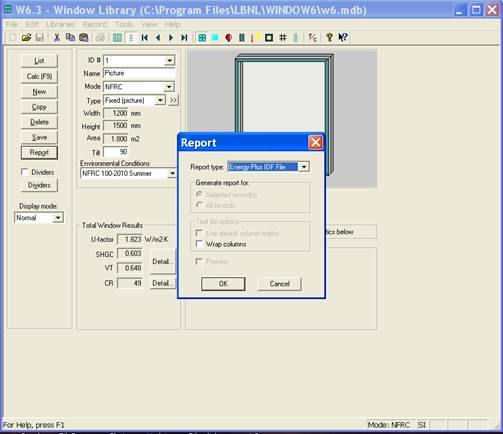
\includegraphics[width=0.9\textwidth, height=0.9\textheight, keepaspectratio=true]{media/image001.jpg}
\caption{WINDOW screen for exporting IDF Window specifications \protect \label{fig:window-screen-for-exporting-idf-window}}
\end{figure}

The file can then be saved at a location of your choice and added into your overall simulation IDF file.

\subsection{WINDOW Data File}\label{window-data-file}

The other ``older'' option for creating data for EnergyPlus is to use the ``EnergyPlus'' option above and create a WindowDataFile. The general format of this data is described in the following paragraphs and must use the Construction:WindowDataFile object and an external file to be used in EnergyPlus. While this is a convenient small file (that can contain multiple windows), there is no way to import this file back into WINDOW and obtain the above, more preferred method.

Please note that there is a bug in WINDOW 5 that causes two of the lines in the EnergyPlus data file to be joined. This bug is fixed in versions of Window 5.02 (and above). To be sure, you can check the data file for a line that looks like:

GLAZING SYSTEM OPTICAL DATA

Angle~~~~ 0~~~ 10~~~ 20~~~ 30~~~ 40~~~ 50~~~ 60~~~ 70~~~ 80~~~ 90 Hemis

The fixed version of the program will not show the above line; rather, there will be two lines such as shown below. If you have the above condition, with an editor you would break this into two lines:

GLAZING SYSTEM OPTICAL DATA

Angle~~~~ 0~~~ 10~~~ 20~~~ 30~~~ 40~~~ 50~~~ 60~~~ 70~~~ 80~~~ 90 Hemis

In EnergyPlus, the Window data file is searched for each ``Construction:WindowDataFile'' object in the EnergyPlus input. This object has a very simple form:

Construction:WindowDataFile,

ConstructionName,

FileName; ! Default is Window5DataFile.dat in the ``run'' folder.

If there is a window called ConstructionName on the Window data file, the data for that window is read from the file and the following EnergyPlus objects and their names are created. The ``W5'' prefixed to these names indicates that the object originated in the Window5 data file.

\begin{itemize}
\item
  \textbf{WindowMaterial:Glazing} for each of the glass layers. They will be named \textbf{W5:ConstructionName:GLASS1}, \textbf{W5:ConstructionName:GLASS2} , etc.
\item
  \textbf{WindowMaterial:Gas} or \textbf{WindowMaterial:GasMixture} for each of the gap layers. They will be named \textbf{W5:ConstructionName:GAP1}, \textbf{W5:ConstructionName:GAP2} , etc.
\item
  \textbf{WindowProperty:FrameAndDivider} (if the window on the Window5 data file has a frame and/or divider). It will be named \textbf{W5:ConstructionName}. This WindowProperty:FrameAndDivider will be assigned to any window on the input file that has a construction called ``ConstructionName'' \emph{even if that window has~ referenced another WindowProperty:FrameAndDivider (i.e., if WindowProperty:FrameAndDivider Name for that window is specified).} In this case a warning will result.
\end{itemize}

Note that:

An entry on the WINDOW data file usually has just one glazing system. It is also possible to have an entry with two glazing systems separated by a horizontal or vertical mullion. In this case, the two glazing systems can have different dimensions and different properties. For example, one of the two glazing systems could be single glazed and the other could be double glazed. An example~ of the two glazing system case is given in the sample WINDOW data file shown below (although in this case the properties of the two glazing systems are the same).

EnergyPlus handles the ``one glazing system'' and ``two glazing systems'' cases differently. If there is one glazing system, the glazing system height and width from the Window5 data file are not used. Instead, the window dimensions are obtained from the window vertices that have been specified on the IDF file. However, a warning message will result if the height or width calculated from the window's vertex inputs differs from the corresponding Window5 data file values by more than 10\%. This warning is given since the effective frame and edge-of-glass conductances on the WINDOW data file can depend on the window dimensions if the frame is non-uniform, i.e., consists of sections with different values of width, projection, or thermal properties.

If the WINDOW data file entry has two glazing systems, System1 and System2, the following happens, as shown in the figure below. Assume that the original window is called WinOriginal. System1 is assigned to WinOriginal. Then EnergyPlus automatically creates a second window, called WinOriginal:2, and assigns System2 to it. The dimensions of WinOriginal are ignored; the dimensions of System1 on the data file are assigned to it, but the position of the lower left-hand vertex of WinOriginal is retained. The dimensions of System2 on the data file are assigned to WinOriginal:2. The lower left-hand vertex of WinOriginal:2 is determined from the mullion orientation and width.

\textbf{Note: WinOriginal would have been the IDF window definition -- it's dimensions will be overridden by the systems dimensions from the Window data file. Two windows will be made and called WinOriginal and WinOriginal:2.}

\begin{figure}[hbtp] % fig 2
\centering
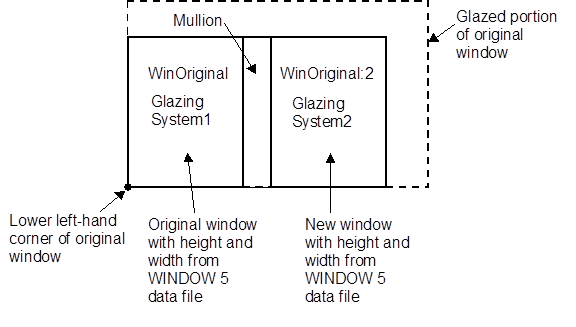
\includegraphics[width=0.9\textwidth, height=0.9\textheight, keepaspectratio=true]{media/image002.png}
\caption{Window Glazing system with dual glazing constructions \protect \label{fig:window-glazing-system-with-dual-glazing}}
\end{figure}

The Window Data File contains no information on shading devices. See ``Specify the Material Name of the Shading Device'' under WindowShadingControl for a method to attach a shading layer to windows read in from this file.

Following is an example WINDOW data file for a slider window with two identical double low-E glazing systems separated by a horizontal mullion. Each system has a frame and divider. Note that all dimensions, such as glazing height and width, are in millimeters; when EnergyPlus reads the file these are converted to meters. Following the data file example is a description of the contents of the file. That data used by EnergyPlus is shown in bold.

Window5 Data File for EnergyPlus

\textless{}WINDOW program version\textgreater{}

Date~~~~~~~~~~~~ : Tue Nov 13 17:07:40 2001

Window name~~~~~ : \textbf{DoubleLowE}

Description~~~~~ : Horizontal Slider, AA

\# Glazing Systems: \textbf{2}

GLAZING SYSTEM DATA: Height Width nPanes Uval-center SC-center SHGC-center Tvis-center

~System1~~~~~~~~ :~~ 1032~~ 669~~~~~ 2~~~~~ 1.660~~~~~ 0.538~~~~~ 0.467~~~~~~ 0.696

~System2~~~~~~~~ :~~ 1033~~ 669~~~~~ 2~~~~~ 1.660~~~~~ 0.538~~ ~~~0.467~~~~~~ 0.696

FRAME/MULLION DATA: Width OutsideProj InsideProj Cond EdgeCondRatio SolAbs VisAbs Emiss~ Orient'n (mull)

~~~ L Sill~~~~~~ :~~ 97.3~~~~ 25.4~~~~~~ 25.4~~ 500.000~~~ 1.467~~~~ 0.500~ 0.500~ 0.90

~~~ R Sill~~~~~~ :~~ 97.3~~~~ 25.4~~~~~~ 25.4~~ 500.000~~~ 1.467~~~~ 0.500~ 0.500~ 0.90

~~~ L Head~~~~~~ :~~ 70.2~~~~ 25.4~~~~~~ 25.4~~ 18.822~~~~ 1.490~~~~ 0.500~ 0.500~ 0.90

~~~ R Head~~~~~~ :~~ 70.2~~~~ 25.4~~~~~~ 25.4~~ 18.822~~~~ 1.490~~~~ 0.500~ 0.500~ 0.90

~~~ Top L Jamb~~ :~~ 54.3~~~~ 25.4~~~~~~ 25.4~~ 31.141~~~~ 1.503~~~~ 0.500~ 0.500~ 0.90

~~~ Bot L Jamb~~ :~~ 54.3~~~~ 25.4~~~~~~ 25.4~~ 500.000~~~ 1.494~~~~ 0.500~ 0.500~ 0.90

~~~ Top R Jamb~~ :~~ 70.2~~~~ 25.4~~~~~~ 25.4~~ 500.000~~~ 1.518~~~~ 0.500~ 0.500~ 0.90

~~~ Bot R Jamb~~ :~~ 97.6 ~~~~25.4~~~~~~ 25.4~~ 264.673~~~ 1.547~~~~ 0.500~ 0.500~ 0.90

~~~ Mullion~~~~~ :~~ 53.5~~~~ 25.4~~~~~~ 25.4~~ 500.000~~~ 1.361~~~~ 0.500~ 0.500~ 0.90 \textbf{Horizontal}

~~~ Average frame:~~ \textbf{75.5~~~~ 25.4~~~~~~ 25.4~~ 326.149~~~ 1.464~~~~ 0.500~ 0.500~ 0.90}

DIVIDER DATA~~~~ : Width OutsideProj InsideProj Cond EdgeCondRatio SolAbs VisAbs Emiss Type~~~~~~~~~~~ \#Hor \#Vert

~System1~~~~~~~~ :~ \textbf{25.4~~~ 25.4~~~~~~ 25.4~~~ 3.068~~~~~ 1.191~~~~ 0.500~ 0.500 0.900 DividedLite~~~~~~ 2~~~ 3}

~System2~~~~~~~~ :~ \textbf{25.4~~~ 25.4~~~~ ~~25.4~~~ 3.068~~~~~ 1.191~~~~ 0.500~ 0.500 0.900 DividedLite~~~~~~ 2~~~ 3}

GLASS DATA~~~~~~ : Layer\#~ Thickness~ Cond Tsol Rfsol Rbsol Tvis Rfvis Rbvis~ Tir~ EmissF~ EmissB~ SpectralDataFile

~System1~~~~~~~~ :~~ 1~~~~~ \textbf{3.00~~~~ 0.900} 0.50~ 0.33~ 0.39 0.78~ 0.16~ 0.13 \textbf{0.00~~ 0.16~~~ 0.13}~~ CMFTIR\_3.AFG

~~~~~~~~~~~~~~~~~~~~ 2~~~~~ \textbf{6.00~~~~ 0.900} 0.77~ 0.07~ 0.07 0.88~ 0.08~ 0.08 \textbf{0.00~~ 0.84~~~ 0.84}~~ CLEAR\_6.DAT

~System2~~~~~~~~ :~~ 1~~~~~ \textbf{3.00~~~~ 0.900} 0.50~ 0.33~ 0.39 0.78~ 0.16~ 0.13 \textbf{0.00~~ 0.16~~~ 0.13}~~ CMFTIR\_3.AFG

~~~~~~~~~~~~~~~~~~~~ 2~~~~~ \textbf{6.00~~~~ 0.900} 0.77~ 0.07~ 0.07 0.88~ 0.08~ 0.08 \textbf{0.00~~ 0.84~~~ 0.84}~~ CLEAR\_6.DAT

GAP DATA~~~~~~~~ : Gap\# Thick nGasses

~System1~~~~~~~~ :~~ 1~ \textbf{12.70~~~ 1}

~System2~~~~~~~~ :~~ 1~ \textbf{12.70~~~ 1}

GAS DATA~~~~~~~~ : GasName Fraction MolWeight ACond~~ BCond~ CCond AVisc~~ BVisc~~ CVisc ASpHeat~ BSpHeat CSpHeat

~System1 Gap1~~~ : Air~~~~ \textbf{1.0000~~ 28.97~~~ 0.002873 7.76e-5 0.0 3.723e-6 4.94e-8 0.0~~ 1002.737 0.012324 0.0}

~System2 Gap1~~~ : Air~~~~ \textbf{1.0000~~ 28.97~~~ 0.002873 7.76e-5 0.0 3.723e-6 4.94e-8 0.0~~ 1002.737 0.012324 0.0}

GLAZING SYSTEM OPTICAL DATA

Angle~~~~ 0~~~ 10~~~ 20~~~ 30~~~ 40~~~ 50~~~ 60~~~ 70~~~ 80~~~ 90 Hemis

System1

Tsol~ \textbf{0.408 0.410 0.404 0.395 0.383 0.362 0.316 0.230 0.106 0.000 0.338}

Abs1~ \textbf{0.177 0.180 0.188 0.193 0.195 0.201 0.218 0.239 0.210 0.001 0.201}

Abs2~ \textbf{0.060 0.060 0.061 0.061 0.063 0.063 0.061 0.053 0.038 0.000 0.059}

Rfsol \textbf{0.355 0.350 0.348 0.350 0.359 0.374 0.405 0.478 0.646 0.999 0.392}

Rbsol \textbf{0.289 0.285 0.283 0.282 0.285 0.296 0.328 0.411 0.594 1.000 0.322}

Tvis~ \textbf{0.696 0.700 0.690 0.677 0.660 0.625 0.548 0.399 0.187 0.000 0.581}

Rfvis \textbf{0.207 0.201 0.198 0.201 0.212 0.234 0.278 0.374 0.582 0.999 0.260}

Rbvis \textbf{0.180 0.174 0.173 0.176 0.189 0.215 0.271 0.401 0.648 1.000 0.251}

System2

Tsol~ \textbf{0.408 0.410 0.404 0.395 0.383 0.362 0.316 0.230 0.106 0.000 0.338}

Abs1~ \textbf{0.177 0.180 0.188 0.193 0.195 0.201 0.218 0.239 0.210 0.001 0.201}

Abs2~ \textbf{0.060 0.060 0.061 0.061 0.063 0.063 0.061 0.053 0.038 0.000 0.059}

Rfsol \textbf{0.355 0.350 0.348 0.350 0.359 0.374 0.405 0.478 0.646 0.999 0.392}

Rbsol \textbf{0.289 0.285 0.283 0.282 0.285 0.296 0.328 0.411 0.594 1.000 0.322}

Tvis~ \textbf{0.696 0.700 0.690 0.677 0.660 0.625 0.548 0.399 0.187 0.000 0.581}

Rfvis \textbf{0.207 0.201 0.198 0.201 0.212 0.234 0.278 0.374 0.582 0.999 0.260}

Rbvis \textbf{0.180 0.174 0.173 0.176 0.189 0.215 0.271 0.401 0.648 1.000 0.251}

\textbf{Description of Contents of WINDOW Data File}

(Quantities used in EnergyPlus are in bold; others are informative only)

Second line = version of WINDOW used to create the data file

\emph{Date} = date the data file was created

\textbf{\emph{Window name}} = name of this window; chosen by WINDOW5 user; EnergyPlus user enters the same name in EnergyPlus as name of a ``Construction from Window5 Data File'' object. EnergyPlus will search the Window5 data file for an entry of this name.

\emph{Description} = One-line description of the window; this is treated as a comment.

\textbf{\emph{\# Glazing Systems}}: 1 or 2; value is usually 1 but can be 2 if window has a horizontal or vertical mullion that separates the window into two glazing systems that may or may not be different.

GLAZING SYSTEM DATA

\emph{System1, System2}: separate characteristics given if window has a mullion.

\textbf{\emph{Height}}, *\textbf{\emph{width}} = height and width of glazed portion (i.e., excluding frame; and, if mullion present, excluding mullion).

\textbf{\emph{nPanes}}~~~~ = number of glass layers

\emph{Uval-center} = center-of-glass U-value (including air films) under standard winter conditions*~ (W/m2)

\emph{SC-center}~~ = center-of-glass shading coefficient under standard summer conditions*.

\emph{SHCG-center} = center-of-glass solar heat gain coefficient under standard summer conditions*.

\emph{Tvis-center} = center-of-glass visible transmittance at normal incidence

FRAME/MULLION DATA

\emph{L,R Sill}~~ = left, right sill of frame

\emph{L,R Head}~~ = left, right header of frame

\emph{Top L, Bot L jamb} = top-left, bottom-left jamb of frame

\emph{Bot L, Bot R jamb} = bottom-left, bottom-right jamb of frame

\textbf{\emph{Average frame}} = average characteristics of frame for use in EnergyPlus calculation. If mullion is present, original window is divided into two separate windows with the same average frame (with the mullion being split lengthwise and included in the average frame).

\textbf{\emph{Width}}~~~~ = width (m)

\textbf{\emph{OutsideProj}} = amount of projection from outside glass (m)

\textbf{\emph{InsideProj}} = amount of projection from inside glass (m)

\textbf{\emph{Cond}} = effective surface-to-surface conductance (from THERM calculation) (W/m2)

\textbf{\emph{EdgeCondRatio}} = ratio of surface-to-surface edge-of-glass conductance to surface-to-surface center-of-glass conductance (from THERM calculation)

\textbf{\emph{SolAbs}}~~~ = solar absorptance

\textbf{\emph{VisAbs}}~~~ = visible absorptance

\textbf{\emph{Emiss}}~~~~ = hemispherical thermal emissivity

\textbf{\emph{Orientation}} = Horizontal or Vertical (mullion only); = None if no mullion.

DIVIDER DATA

\textbf{\emph{Width}} through \textbf{\emph{Emiss}} are the same as for FRAME/MULLION DATA

\textbf{\emph{\#Hor}}~~~~~ = number of horizontal dividers

\textbf{\emph{\#Vert}}~~~~ = number of vertical dividers

\textbf{\emph{Type}}~~~~~ = DividedLite or Suspended

GLASS DATA

\emph{System1, System2}: separate characteristics are given if window has a mullion.

\textbf{\emph{Cond}}~~~~~~ = conductivity (W/m-K)

\emph{Tsol}~~~~~~ = spectral-average solar transmittance at normal incidence

\emph{Rfsol}~~~~~ = spectral-average front solar reflectance at normal incidence

\emph{Rbsol}~~~~~ = spectral-average back solar reflectance at normal incidence

\emph{Tvis}~~~~~~ = spectral-average visible transmittance at normal incidence

\emph{Rfvis}~~~~~ = spectral-average front visible reflectance at normal incidence

\emph{Rbvis}~~~~~ = spectral-average back visible reflectance at normal incidence

\textbf{\emph{Tir}}~~~~~~ = hemispherical IR transmittance

\textbf{\emph{EmissF}}~~~ = hemispherical front emissivity

\textbf{\emph{EmissB}}~~~ = hemispherical back emissivity

SpectralDataFile = name of spectral data file with wavelength-dependent transmission and reflection data used by WINDOW 5 to calculate the glazing system optical data. ``None'' will appear here if spectral-average data for this glass layer were used by WINDOW 5.

GAP DATA

System1, System2: separate characteristics are given if the window has a mullion.

\textbf{\emph{Thick}}~~~~ = thickness (m)

\textbf{\emph{nGasses}}~ = number of gasses (1, 2 or 3)

GasName~~ = name of the gas

\textbf{\emph{Fraction}}~ = fraction of the gas

\textbf{\emph{MolecWeight}} = molecular weight of the Nth gas

(In the following, conductivity, viscosity and specific heat as a function

of temperature, T (deg K), are expressed as A + B*T + C*T\^{}2)

\textbf{\emph{ACond}}~~~~ = A coeff of conductivity (W/m-K)

\textbf{\emph{BCond}}~~~~ = B coeff of conductivity (W/m-K\^{}2)

\textbf{\emph{CCond}}~~~~ = C coeff of conductivity (W/m-K\^{}3)

\textbf{\emph{AVisc}}~~~~ = A coeff of viscosity (g/m-s)

\textbf{\emph{BVisc}}~~~~ = B coeff of viscosity (g/m-s-K)

\textbf{\emph{CVisc}}~~~~ = C coeff of viscosity (g/m-s-K\^{}2)

\textbf{\emph{ASpHeat}}~~ = A coeff of specific heat (J/kg-K)

\textbf{\emph{BSpHeat}}~~ = B coeff of specific heat (J/kg-K\^{}2)

\textbf{\emph{CSpHeat}}~~ = C coeff of specific heat (J/kg-K\^{}3)

GLAZING SYSTEM OPTICAL DATA

System1, System2: separate characteristics are given if the window has a mullion.

\textbf{\emph{Hemisph}}~~ = hemispherical (i.e., diffuse)

\textbf{\emph{Tsol}}~~~~~ = solar transmittance vs.~angle of incidence

\textbf{\emph{AbsN}}~~~~~ = solar absorptance of Nth layer vs.~angle of incidence

\textbf{\emph{Rfsol}}~~~~ = front solar reflectance vs.~angle of incidence

\textbf{\emph{Rbsol}}~~~~ = back solar reflectance vs.~angle of incidence

\textbf{\emph{Tvis}}~~~~~ = visible transmittance vs.~angle of incidence

\textbf{\emph{Rfvis}}~~~~ = front visible reflectance vs.~angle of incidence

\textbf{\emph{Rbvis}}~~~~ = back visible reflectance vs.~angle of incidence

\begin{center}\rule{0.5\linewidth}{0.4pt}\end{center}

*Standard conditions are

~ Winter:

~ Indoor air temperature = 21.1C (70F)

~ Outdoor air temperature = -17.8C (0F)

~ Wind speed = 6.71 m/s (15 mph)

~ No solar radiation

~ Summer:

~ Indoor air temperature = 23.9C (75F)

~ Outdoor air temperature = 31.7C (89F)

~ Wind speed = 3.35 m/s (7.5 mph)

~ 783 W/m2 (248 Btu/h-ft2) incident beam solar radiation normal to glazing


\chapter{Building Geometry, Shading \& Zone Model}\label{building-geometry-shading-zone-model}


\section{Building Surface Dimensions -- Inside, Outside or Centerline}\label{building-surface-dimensions-inside-outside-or-centerline}

When describing the geometry of building surfaces in EnergyPlus, all surfaces are a thin plane without any thickness. The thickness property of the materials which are assigned to the building surface are only used for heat conduction and thermal mass calculations. Because EnegyPlus geometry is represented with a thin plane, which actual dimension is the proper one to use: inside, outside, or centerline dimensions. For most buildings, the difference is small, and the user may use whatever dimensions are most convenient. A suggested approach is to use outside dimensions for exterior surfaces, and centerline dimensions for interior surfaces. This produces fully connected geometry with an appropriate amount of floor area, zone volume, and thermal mass. If desired, zone volume and floor area may be overridden by entering values in the Zone object. For buildings with very thick walls, such as centuries-old masonry buildings, it is recommended that centerline dimensions be used for all surfaces (exterior and interior) so that the model will have the correct amount of thermal mass.


\section{Describing Roof Overhangs}\label{describing-roof-overhangs}

Building heat transfer surfaces, such as roofs and walls, only cast shadows in a hemisphere in the direction of the outward facing normal (see Figure~\ref{fig:building-heat-transfer-surfaces-cast-shadows}). Because roof surfaces generally face upward, a roof surface which extends beyond the walls of the building will not cast shadows on the walls below it (see Figure~\ref{fig:extended-roof-surface-will-not-shade}).

\begin{figure}[hbtp] % fig 3
\centering
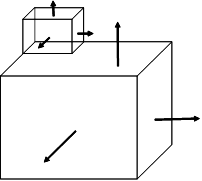
\includegraphics[width=0.9\textwidth, height=0.9\textheight, keepaspectratio=true]{media/image003.png}
\caption{Building heat transfer surfaces cast shadows in the direction of outward facing normal. \protect \label{fig:building-heat-transfer-surfaces-cast-shadows}}
\end{figure}

\begin{figure}[hbtp] % fig 4
\centering
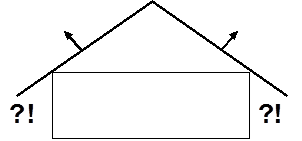
\includegraphics[width=0.9\textwidth, height=0.9\textheight, keepaspectratio=true]{media/image004.png}
\caption{Extended roof surface will not shade the walls below. \protect \label{fig:extended-roof-surface-will-not-shade}}
\end{figure}

Figure~\ref{fig:proper-surface-configurations-for-roof} shows the proper surface configurations for two types of attic construction. In all cases, the roof surface should only include the area of the roof which contacts the zone below it. In these drawings, this is an unconditioned attic space, but it could also be a conditioned zone. Any extensions of the roof which are exposed to the outdoors on both sides should be described as a shading surface.

For the configuration on the left, the overhang should be a shading surface which will cast shadows in both directions (if the default mirroring is disabled the shading surface must face downward). This ensures that the correct shading will be modeled, and it also avoids overstating the heat transfer through the roof into the attic.

For the configuration on the right, the attic is fully enclosed with building heat transfer surfaces for the roof and soffits. The soffits would be described as floor surfaces in the attic and would face downward. The central portion of the attic floor would be described as an interzone floor surface where the outside boundary condition is the ceiling surface in the zone below.

\begin{figure}[hbtp] % fig 5
\centering
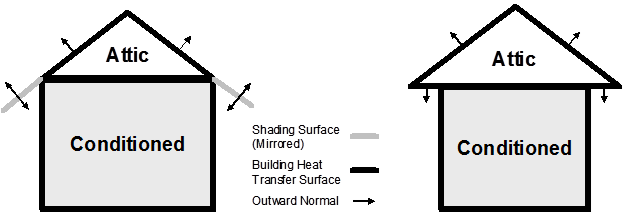
\includegraphics[width=0.9\textwidth, height=0.9\textheight, keepaspectratio=true]{media/image005.png}
\caption{Proper surface configurations for roof overhangs for two types of attic construction. \protect \label{fig:proper-surface-configurations-for-roof}}
\end{figure}


\section{Solar Reflection from Shading Surfaces}\label{solar-reflection-from-shading-surfaces}

Exterior shading surfaces modeled using ``FullInteriorAndExteriorWithReflections'' can show some sky diffuse solar getting through the shades. When ``*WithReflections'' is active a partially sunlit shading surface reflects uniformly from the entire surface. If using WithReflections, shading surfaces should be broken into multiple surfaces at lines of intersection with other shading surfaces. This also includes places where another surface may tee into a shading surface.

For example, a building is shaded by surfaces A, B, and C. Shading Surface A intercepts with Shading Surfaces B and C, and are broken into three areas A1, A2, and A3. Surface A should be entered as the shown three shading areas in order to correctly model sky diffuse solar reflection from Shading Surface A.

\begin{figure}[hbtp] % fig 6
\centering
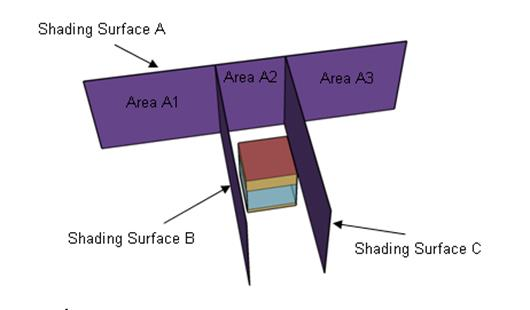
\includegraphics[width=0.9\textwidth, height=0.9\textheight, keepaspectratio=true]{media/image006.jpg}
\caption{Limitations in modeling reflections from surfaces \protect \label{fig:limitations-in-modeling-reflections-from}}
\end{figure}


\section{Air wall, Open air connection between zones}\label{air-wall-open-air-connection-between-zones}

Modeling the interactions between thermal zones which are connected by a large opening requires special consideration. EnergyPlus models only what is explicitly described in the input file, so simply leaving a void (no surfaces) between two zones will accomplish nothing - the two zones will not be connected. A building surface or fenestration surface with Construction:AirBoundary may be used connect the zones. Construction:AirBoundary has options for modeling the interactions which occur across the dividing line between two zones which are fully open to each other:

\begin{description}
  \item[Convection or airflow] transfers both sensible heat and moisture. Some modelers use ZoneMixing (one-way flow) or ZoneCrossMixing (two-way flow) to move air between the zones, but the user must specify airflow rates and schedules for this flow. Other modelers use AirFlowNetwork with large openings between the zones as well as other openings and cracks in the exterior envelope to provide the driving forces. ZoneMixing flows can be linked to HVAC system operation using ZoneAirMassFlowConservation or AirflowNetwork:Distribution:*. Construction:AirBoundary has an option to automatically add a pair of ZoneMixing objects.

  \item[Solar gains and daylighting] gains in perimeter zones often project into a core zone across an open air boundary. Normally, the only way to pass solar and daylight from one zone to the next is through a window or glass door described as a subsurface on an interzone wall surface. Note that all solar is diffuse after passing through an interior window. Construction:AirBoundary groups adjacent zones into a common enclosure for solar and daylighting distribution allowing both direct and diffuse solar (and daylighting) to pass between the adjacent zones.

  \item[Radiant (long-wave thermal) transfer] can be signifcant between exterior surfaces of a perimeter zone and interior surfaces of a core zone with an open boundary between them. Normally, there is no direct radiant exchange between surfaces in different thermal zones. Construction:AirBoundary groups adjacent zones into a common enclosure for radiant exchange, allowing surfaces in different zones to ``see'' each other.

  \item[Visible and thermal radiant output] from internal gains will not normally cross zone boundaries. Construction:AirBoundary will distribute these gains across all surfaces in the grouped enclosure.
\end{description}



\section{Daylight Modeling}\label{daylight-modeling}

\emph{Why isn't my lighting energy being reduced with a daylighting system?}

In order to see changes in the lighting electric power consumption due to daylighting, the Fraction Replaceable in the \textbf{Lights} input object must be set to 1.0. This is documented in the I/O reference, and also a warning is generated in the ERR file.


\section{Rain Flag}\label{rain-flag}

\emph{Why is my exterior convection coefficient value 1000?}

When the outside environment indicates that it is raining, the exterior surfaces (exposed to wind) are assumed to be wet. The convection coefficient is set to a very high number (1000) and the outside temperature used for the surface will be the wet-bulb temperature. (If you choose to report this variable, you will see 1000 as its value.)


\section{Interzone Exterior Convection}\label{interzone-exterior-convection}

\emph{Why is my exterior convection coefficient value 0?}

When two surfaces are linked as interzone surfaces, the ``exterior'' side of these surfaces does not really exist. EnergyPlus links the two surfaces by using the inside temperature of surface A as the outside temperature of surface B, and the reverse. For example:

Zone1WestWall has an outside boundary of Surface = Zone2EastWall

Zone2EastWall has an outside boundary of Surface = Zone1WestWall

Let's say that at hour 2, the inside surface temperature of Zone1WestWall is 19C, and the inside temperature of Zone2EastWall is 22C. When the heat balance is calculated for Zone1WestWall, its outside surface temperature will be set to 22C. Likewise, when the heat balance is calculated for Zone2EastWall, its outside surface temperature will be set to 19C. So, for interzone surfaces, h ext does not apply. That is why it is reported as zero.


\section{Modeling Reflective Radiant Barriers}\label{modeling-reflective-radiant-barriers}

\emph{Can EnergyPlus model reflective radiant barriers?}

\begin{enumerate}
\def\labelenumi{\arabic{enumi}.}
\tightlist
\item
  For radiant barriers which are exposed to a thermal zone, such as an attic space, specify a reduced thermal absorptance for the innermost material layer.
\end{enumerate}

For example, an attic roof construction might be (outer to inner)

\begin{lstlisting}

Asphalt shingles,
  R-30 insulation,
  Radiant barrier;
\end{lstlisting}

The radiant barrier material would be a thin layer with some small resistance with a low thermal absorptance value. This will reduce the radiant heat transfer from the roof surface to other surfaces in the attic zone.

\begin{enumerate}
\def\labelenumi{\arabic{enumi}.}
\setcounter{enumi}{1}
\tightlist
\item
  If the radiant barrier is within a cavity which is not modeled as a separate thermal zone, then there is not an easy way to model its impact. For example, a wall construction:
\end{enumerate}

\begin{lstlisting}

Brick,
  R-12 insulation,
  Radiant barrier,
  Air gap,
  Gypsum board;
\end{lstlisting}

Here, the radiant barrier would reduce the radiant transfer across the air gap. But EnergyPlus air gaps are a fixed thermal resistance, specified in the Material:Airgap object. The user would need to compute an average effective resistance which represents the reduced radiant heat transfer across the air gap due to the radiant barrier. This resistance could then be assigned to the radiant barrier material layer.


\section{Cavity Algorithm Model}\label{cavity-algorithm-model}

\emph{Reading the documentation, I'm wondering if the Cavity algorithm is usable for other double facade types or only Trombe wall?~ In other words, does Cavity implicitly presume that the inner wall is highly solar absorbent and so generate specific convection?}

The Trombe wall convection algorithm is applicable to just about any vertical cavity with a high aspect ratio and relatively narrow width. I'm not sure if a double facade cavity would meet the aspect ratio requirement. But I do know the Trombe wall algorithm is not picky about whether the inner wall is highly absorbant, or about any particular properties of the walls. Actually the same basic algorithm is used by the window model to calculate the convection between the two panes of a window. The full reference is ISO 15099.


\section{Using Multipliers (Zone and/or Window)}\label{using-multipliers-zone-andor-window}

\subsection{Background and Study using Multipliers}\label{background-and-study-using-multipliers}

Multipliers are used in EnergyPlus for convenience in modeling. Though window multipliers are useful for any size building when you have multiple windows on a façade, zone multipliers are more useful in large buildings with several to many stories.

Zone multipliers are designed as a ``multiplier'' for floor area, zone loads, and energy consumed by internal gains. It takes the calculated load for the zone and multiplies it, sending the multiplied load to the attached HVAC system. The HVAC system size is specified to meet the entire multiplied zone load and will report the amount of the load met in the Zone/Sys Sensible Heating or Cooling Energy/Rate report variable. Autosizing automatically accounts for multipliers. Metered energy consumption by internal gains objects such as Lights or Electric Equipment will be multiplied.

To illustrate the benefits (and comparison of results), the MultiStory.idf example file was used. The MultiStory file is a 9 zone, 10 story/floored building with heating (ZoneHVAC:Baseboard:Convective:Electric object) and cooling (ZoneHVAC:WindowAirConditioner object). The middle zone of each floor in the original represents 4 zones (multiplier = 4) and the middle floor (ZoneGroup) represents 8 floors (ZoneGroup multiplier = 8). Clone representations were made for comparisons:

\begin{figure}[hbtp] % fig 7
\centering
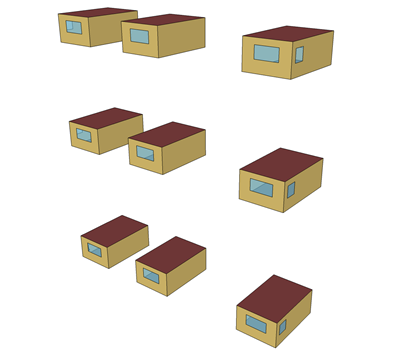
\includegraphics[width=0.9\textwidth, height=0.9\textheight, keepaspectratio=true]{media/image007.png}
\caption{Original Multistory IDF \protect \label{fig:original-multistory-idf}}
\end{figure}

In the figure above, each ``middle'' zone represents 4 zones.~ The middle ``floor'' represents 8 floors. Additionally, each of the windows has a multiplier of 4 -- so each window represents 4 windows of the same size. For the Multistory file, the Zone object for the center zones has the multiplier of 4. And for the center floors, the ZoneList and ZoneGroup objects to collect the zones and apply multipliers. The top floor then uses the Zone object multiplier for the center zones. Specifically:

\begin{lstlisting}

<snip>
    Zone,
      Gnd Center Zone,         !- Name
      0.0,                     !- Direction of Relative North {deg}
      8.0, 0.0, 0.0,           !- Origin [X,Y,Z] {m}
      1,                       !- Type
      4,                       !- Multiplier
      autocalculate,           !- Ceiling Height {m}
      autocalculate;           !- Volume {m3}
  <snip>

    ZoneGroup,
      Mid Floor,               !- Zone Group Name
      Mid Floor List,          !- Zone List Name
      8;                       !- Zone List Multiplier


    ZoneList,
      Mid Floor List,          !- Zone List Name
      Mid West Zone,           !- Zone 1 Name
      Mid Center Zone,         !- Zone 2 Name
      Mid East Zone;           !- Zone 3 Name
  <snip>

    Zone,
      Top Center Zone,         !- Name
      0.0,                     !- Direction of Relative North {deg}
      8.0,                     !- X Origin {m}
      0.0,                     !- Y Origin {m}
      22.5,                    !- Z Origin {m}
      1,                       !- Type
      4,                       !- Multiplier
      autocalculate,           !- Ceiling Height {m}
      autocalculate;           !- Volume {m3}
\end{lstlisting}

For comparison purposes, clones of the middle zones were done.

\begin{figure}[hbtp] % fig 8
\centering
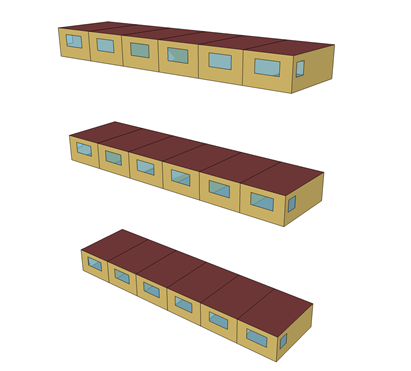
\includegraphics[width=0.9\textwidth, height=0.9\textheight, keepaspectratio=true]{media/image008.png}
\caption{Multistory with cloned middle zones. \protect \label{fig:multistory-with-cloned-middle-zones.}}
\end{figure}

And, finally, the entire building was created:

\begin{figure}[hbtp] % fig 9
\centering
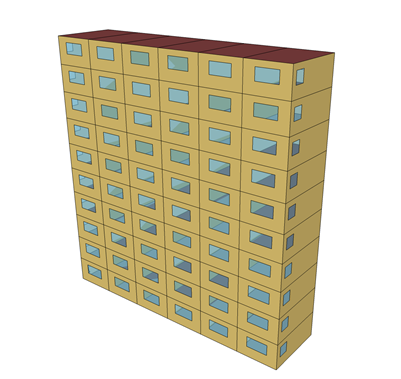
\includegraphics[width=0.9\textwidth, height=0.9\textheight, keepaspectratio=true]{media/image009.png}
\caption{Multistory building -- fully cloned. \protect \label{fig:multistory-building-fully-cloned.}}
\end{figure}

The building is autosized. For convenience in comparison, the extreme summer and winter days were used for autosizing and the simulation was run for the 5 United States weather files that are included in the EnergyPlus release: Chicago IL; San Francisco CA; Golden CO; Tampa FL; and Washington DC.

Comparisons were done with the Zone Group Loads values (Zone Group Sensible Heating Energy and Zone Group Sensible Cooling Energy) as well as meter values for Electricity. Using the regression testing limits that are used during EnergyPlus development testing (i.e.~small differences are within .001 or .5\%; big differences are greater than those limits).

For the purposes of dicussion, the buildings will be called: Multistory 1 -- the original 9 zone building (with multipliers and groups) ref: Figure~\ref{fig:original-multistory-idf}; Multistory 2 -- the building shown in Figure~\ref{fig:multistory-with-cloned-middle-zones.}. Multistory with cloned middle zones.; Multistory 3 -- the fully configured building -- ref Figure~\ref{fig:multistory-building-fully-cloned.}.

The following table illustrates the regression testing for Multistory 2 and Multistory 3, group loads and meters versus Multistory 1 results.

% table 1
\begin{longtable}[c]{p{1.2in}p{1.2in}p{1.2in}p{1.2in}p{1.2in}}
\caption{Multistory vs Multistory 2 and Multistory 3 \label{table:multistory-vs-multistory-2-and-multistory-3}} \tabularnewline
\toprule 
LOCATION & MULTI-STORY 2 LOADS & MULTI-STORY 2 METER & MULTI-STORY 3 LOADS & MULTI-STORY 3 METER \tabularnewline
\midrule
\endfirsthead

\caption[]{Multistory vs Multistory 2 and Multistory 3} \tabularnewline
\toprule 
LOCATION & MULTI-STORY 2 LOADS & MULTI-STORY 2 METER & MULTI-STORY 3 LOADS & MULTI-STORY 3 METER \tabularnewline
\midrule
\endhead

USA\_IL\_Chicago-OHare.Intl.AP.725300\_TMY3 & Small Diffs & Equal & Big Diffs* (76\%) & Big Diffs* (62\%) \tabularnewline
USA\_CA\_San.Francisco.Intl.AP.724940\_TMY3 & Big Diffs* (2.43\%) & Big Diffs* (0.6\%) & Big Diffs* (49\%) & Big Diffs* (41\%) \tabularnewline
USA\_CO\_GOLDEN-NREL.724666\_TMY3 & Small Diffs & Small Diffs & Big Diffs* (26\%) & Big Diffs* (24\%) \tabularnewline
USA\_FL\_Tampa.Intl.AP.722110\_TMY3 & Small Diffs & Small Diffs & Big Diffs* (6\%) & Big Diffs* (2\%) \tabularnewline
USA\_VA\_Sterling-Washington.Dulles.Intl.AP.724030\_TMY3 & Equal & Equal & Big Diffs* (91\%) & Big Diffs* (72\%) \tabularnewline
\bottomrule
\end{longtable}

* Big Diffs maximum occur in monthly values whereas the runperiod values are much smaller.

To try to pare down the discrepancies shown here, the effects of height that are used in the calculations were removed (i.e., the Site:WeatherStation and Site:HeightVariation objects were entered as below to negate the effects of height on the environmental variables such as wind and temperature).~ In addition the height effect was removed from the OutdoorAir:Node object.

\begin{lstlisting}

  Site:WeatherStation,
      ,          !- Wind Sensor Height Above Ground {m}
      ,          !- Wind Speed Profile Exponent
      ,          !- Wind Speed Profile Boundary Layer Thickness {m}
      0;         !- Air Temperature Sensor Height Above Ground {m}


    Site:HeightVariation,
      0,         !- Wind Speed Profile Exponent
      ,          !- Wind Speed Profile Boundary Layer Thickness {m}
      0;         !- Air Temperature Gradient Coefficient {K/m}
\end{lstlisting}

Figure 10. Objects removing height from building impacts.

With these included, the files were rerun with the following results:

% table 2
\begin{longtable}[c]{p{1.2in}p{1.2in}p{1.2in}p{1.2in}p{1.2in}}
\caption{Multiplier Results with negated height variation. \label{table:multiplier-results-with-negated-height}} \tabularnewline
\toprule 
Location & Multi-story 2 Loahs & Multi-story 2 Meter & Multi-story 3 Loahs & Multi-story 3 Meter \tabularnewline
\midrule
\endfirsthead

\caption[]{Multiplier Results with negated height variation.} \tabularnewline
\toprule 
Location & Multi-story 2 Loahs & Multi-story 2 Meter & Multi-story 3 Loahs & Multi-story 3 Meter \tabularnewline
\midrule
\endhead

USA\_IL\_Chicago-OHare.Intl.AP.725300\_TMY3 & Small diffs & Small diffs & Small diffs & Small diffs \tabularnewline
USA\_CA\_San.Francisco.Intl.AP.724940\_TMY3 & Small diffs & Small diffs & Small diffs & Small diffs \tabularnewline
USA\_CO\_GOLDEN-NREL.724666\_TMY3 & Small diffs & Small diffs & Small diffs & Small diffs \tabularnewline
USA\_FL\_Tampa.Intl.AP.722110\_TMY3 & Small diffs & Small diffs & Small diffs & Small diffs \tabularnewline
USA\_VA\_Sterling-Washington.Dulles.Intl.AP.724030\_TMY3 & Small diffs & Small diffs & Small diffs & Small diffs \tabularnewline
\bottomrule
\end{longtable}

To investigate if other systems might have different results, the Ideal Loads System was used as the system.~ Similar results were found for the multipliers vs cloned results. However, it may also be noted that the results between the original systems (baseboard and window ac) vs the ideal loads were very similar.

The biggest difference really comes in calculation time. As shown in the following table,

% table 3
\begin{longtable}[c]{p{1.5in}p{1.5in}p{1.5in}p{1.5in}}
\caption{Runtimes for Multistory files (baseboard/window ac) \label{table:runtimes-for-multistory-files-baseboardwindow}} \tabularnewline
\toprule 
Location & Multi-story 1 (9 zones) (mm:ss) & Multi-story 2~ (18 zones) (MM:SS) & Multi-story 3 (60 zones) (MM:SS) \tabularnewline
\midrule
\endfirsthead

\caption[]{Runtimes for Multistory files (baseboard/window ac)} \tabularnewline
\toprule 
Location & Multi-story 1 (9 zones) (mm:ss) & Multi-story 2~ (18 zones) (MM:SS) & Multi-story 3 (60 zones) (MM:SS) \tabularnewline
\midrule
\endhead

USA\_IL\_Chicago-OHare.Intl.AP.725300\_TMY3 & 1:05 & 2:14 & 13:15 \tabularnewline
USA\_CA\_San.Francisco.Intl.AP.724940\_TMY3 & 1:04 & 2:05 & 13:20 \tabularnewline
USA\_CO\_GOLDEN-NREL.724666\_TMY3 & 1:17 & 2:28 & 14:43 \tabularnewline
USA\_FL\_Tampa.Intl.AP.722110\_TMY3 & 1:11 & 2:21 & 13:43 \tabularnewline
USA\_VA\_Sterling-Washington.Dulles.Intl.AP.724030\_TMY3 & 1:05 & 2:15 & 13:18 \tabularnewline
\bottomrule
\end{longtable}

Because the overall results were so similar, the run times for the Ideal Loads runs are included:

% table 4
\begin{longtable}[c]{p{1.5in}p{1.5in}p{1.5in}p{1.5in}}
\caption{Runtime for Multistory files (ideal loads) \label{table:runtime-for-multistory-files-ideal-loads}} \tabularnewline
\toprule 
Location & Multi-story 1 (9 zones) (mm:ss) & Multi-story 2 (18 zones) (MM:SS) & Multi-story 3 (60 zones) (MM:SS) \tabularnewline
\midrule
\endfirsthead

\caption[]{Runtime for Multistory files (ideal loads)} \tabularnewline
\toprule 
Location & Multi-story 1 (9 zones) (mm:ss) & Multi-story 2 (18 zones) (MM:SS) & Multi-story 3 (60 zones) (MM:SS) \tabularnewline
\midrule
\endhead

USA\_IL\_Chicago-OHare.Intl.AP.725300\_TMY3 & 0:51 & 1:34 & 9:37 \tabularnewline
USA\_CA\_San.Francisco.Intl.AP.724940\_TMY3 & 0:50 & 1:34 & 9:59 \tabularnewline
USA\_CO\_GOLDEN-NREL.724666\_TMY3 & 0:51 & 1:40 & 10:31 \tabularnewline
USA\_FL\_Tampa.Intl.AP.722110\_TMY3 & 0:51 & 1:36 & 10:05 \tabularnewline
USA\_VA\_Sterling-Washington.Dulles.Intl.AP.724030\_TMY3 & 0:51 & 1:36 & 9:48 \tabularnewline
\bottomrule
\end{longtable}

More zones (and, particularly more surfaces) make for longer run times.

\subsection{Guidelines for Using Multipliers and Groups}\label{guidelines-for-using-multipliers-and-groups}

\begin{itemize}
\item
  If the basic zone geometry is identical, make one zone, copy \& paste it as necessary, then change the Zone Origin field to locate each zone correctly.
\item
  Do not use interzone surfaces between zones that are multiplied. Set the adjoining surfaces to be adiabatic, i.e.~use the OtherZoneSurface exterior boundary condition with the other surface pointing back to itself.
\item
  Locate the middle floor zones roughly halfway between top and ground because exterior convection coefficients change with height. Halfway should cause the differences to average out. If you have many stories (the example only has 10 stories), consider using more middle floor zones.
\item
  Consider removing the effects of height variation for the simulation.
\item
  Follow guidelines in HVACTemplate and other objects about sizing if you are mixing autosize fields with hard sized fields (recommended to ``autosize'' all fields rather than mix).
\item
  All HVAC system sizes must be specified to meet the entire multiplied zone load.
\item
  Autosizing automatically accounts for multipliers.
\end{itemize}


\section{Using OSC (Other Side Coefficients) to create controlled panels}\label{using-osc-other-side-coefficients-to-create-controlled-panels}

The Other Side Coefficient (OSC) equation permits setting either the outside surface temperature or the outside air temperature to a constant value or a scheduled value based on the size of the first input parameter, N1. The original temperature equation was:

\begin{equation}
T = N_2 T_{zone} + N_3 T_{oadb} + N_4 N_5 + N_6 T_{grnd} + N_7 W_{spd} T_{oadb}
\end{equation}

where:

\begin{itemize}
\item
  \(T\) = Outside Air Temperature when N1 (Combined convective/radiative film Coeff) \textgreater{} 0
\item
  \(T\) = Exterior Surface Temperature when N1 (Combined convective/radiative film Coeff) \textless{} = 0
\item
  \(T_{zone}\) = MAT = Temperature of the zone being simulated (°C)
\item
  \(T_{oadb}\) = Dry-bulb temperature of the outdoor air (°C)
\item
  \(T_{grnd}\) = Temperature of the ground (°C) Wspd = Outdoor wind speed (m/sec)
\end{itemize}

The coefficients N\(_{2}\), N\(_{3}\), N\(_{4}\), N\(_{6}\), and N\(_{7}\) scale the contribution of the various terms that follow them.~ In the case of N\(_{4}\), it is followed by another term N\(_{5}\).~ This is a constant temperature that can also be overridden by a scheduled value. Note that in some EnergyPlus documentation, the N's are given as C's.

This object has been changed to permit the outside temperature, T, to be controlled to a set point temperature that is specified as N\(_{5}\) or comes from the schedule A2.

Note that since the surface that contains the panel subsurfaces (that must be called doors in EnergyPlus) receives that same outside temperature as the panels, it should have a construction with a very high thermal resistance to essentially take it out of the room heat balance calculation.

An Example input file object is shown below.

\begin{lstlisting}

SurfaceProperty:OtherSideCoefficients,
     Zn001:Roof001:OSC, !- Name
     0,   ! (N1) Combined Convective/Radiative Film Coefficient {W/m2-K}
     0,   ! (N5) Constant Temperature {C}
     0.95,!(N4) Constant Temperature Coefficient
     ,    ! (N3)External Dry-Bulb Temperature Coefficient
     ,    ! (N6)Ground Temperature Coefficient
     ,    ! (N7)Wind Speed Coefficient
     -.95,! (N2) Zone Air Temperature Coefficient
     ConstantCooling,     ! (A2) Constant Temperature Schedule Name
     No,  ! (A3)Sinusoidal Variation of Constant Temperature Coefficient
     24,  ! (N8)Period of Sinusoidal Variation {hr}
     1.,  ! (N9)Previous Other Side Temperature Coefficient
     5.,  !(N10) Minimum Other Side Temperature Limit
     25.; ! (N11) Maximum Other Side Temperature Limit
\end{lstlisting}

This object results in the following equation for T:

T = 1.0*Tlast +0.95*(Tsetpoint -- TzoneAir)~~ (with limits)

The result of this is that the surface temperature, T, will be changed to the temperature that will force the zone air temperature to the setpoint providing the temperature limits are not reached. When the zone air temperature is at the setpoint, T remains at the value it had in the prior time step.

A complete example with all pertinent objects:

\begin{lstlisting}

  Construction,
      PanelConst,              !- Name
      Std Steel_Brown_Regular; !- Outside Layer


    Material,
      Std Steel_Brown_Regular, !- Name
      Smooth,                  !- Roughness
      1.5000000E-03,           !- Thickness {m}
      44.96960,                !- Conductivity {W/m-K}
      7689.000,                !- Density {kg/m3}
      418.0000,                !- Specific Heat {J/kg-K}
      0.9000000,               !- Thermal Absorptance
      0.9200000,               !- Solar Absorptance
      0.92000000;              !- Visible Absorptance


    BuildingSurface:Detailed,
      Zn001:Roof001,           !- Name
      Roof,                    !- Surface Type
      ROOF31,                  !- Construction Name
      ZONE ONE,                !- Zone Name
      OtherSideCoefficients,   !- Outside Boundary Condition
      Zn001:Roof001:OSC,       !- Outside Boundary Condition Object
      NoSun,                   !- Sun Exposure
      NoWind,                  !- Wind Exposure
      0,                       !- View Factor to Ground
      4,                       !- Number of Vertices
      0.000000,15.24000,4.572,  !- X,Y,Z = = > Vertex 1 {m}
      0.000000,0.000000,4.572,  !- X,Y,Z = = > Vertex 2 {m}
      15.24000,0.000000,4.572,  !- X,Y,Z = = > Vertex 3 {m}
      15.24000,15.24000,4.572;  !- X,Y,Z = = > Vertex 4 {m}


    FenestrationSurface:Detailed,
      panel002,                !- Name
      Door,                    !- Surface Type
      PanelConst,              !- Construction Name
      Zn001:Roof001,           !- Building Surface Name
      ,                        !- Outside Boundary Condition Object
      autocalculate,           !- View Factor to Ground
      ,                        !- Frame and Divider Name
      1,                       !- Multiplier
      4,                       !- Number of Vertices
      3,2,4.572,  !- X,Y,Z = = > Vertex 1 {m}
      3,3,4.572,  !- X,Y,Z = = > Vertex 2 {m}
      4,3,4.572,  !- X,Y,Z = = > Vertex 3 {m}
      4,2,4.572;  !- X,Y,Z = = > Vertex 4 {m}


    SurfaceProperty:OtherSideCoefficients,
      Zn001:Roof001:OSC,       !- Name
      0,            !- Combined Convective/Radiative Film Coefficient {W/m2-K}
      0,                       !- Constant Temperature {C}
      0.95,                    !- Constant Temperature Coefficient
      ,                        !- External Dry-Bulb Temperature Coefficient
      ,                        !- Ground Temperature Coefficient
      ,                        !- Wind Speed Coefficient
      -.95,                    !- Zone Air Temperature Coefficient
      ConstantTwentyTwo,       !- Constant Temperature Schedule Name
      No,           !- Sinusoidal Variation of Constant Temperature Coefficient
      24,                      !- Period of Sinusoidal Variation {hr}
      1.,                      !- Previous Other Side Temperature Coefficient
      5.,                      !- Minimum Other Side Temperature Limit {C}
      25.;                     !- Maximum Other Side Temperature Limit {C}


  Schedule:Constant,ConstantTwentyTwo,PanelControl,22;
\end{lstlisting}


\chapter{Natural and Mechanical Ventilation}\label{natural-and-mechanical-ventilation}


\section{AirflowNetwork and EarthTube}\label{airflownetwork-and-earthtube}

\emph{When I use an Earthtube with an AirFlowNetwork, I get a ``Orphan Object'' warning.}

Currently, Earthtube and AirFlowNetworks do not work together.~ If both objects co-exist, the AirflowNetwork mode supersedes the Earthtube mode at two control choices. Since this causes the Earthtube objects to not be used, the ``orphan'' warning appears.

There are four control choices in the second field of the AirflowNetwork Simulation object (spaces included for readability)

\begin{itemize}
\item
  MULTIZONE WITH DISTRIBUTION
\item
  MULTIZONE WITHOUT DISTRIBUTION
\item
  MULTIZONE WITH DISTRIBUTION ONLY DURING FAN OPERATION
\item
  NO MULTIZONE OR DISTRIBUTION
\end{itemize}

When the first two choices are selected, the AirflowNetwork model takes over airflow calculation. The earthtube objects are not used in the airflow calculation, causing the ``orphan'' warning. The example file, AirflowNetwork\_Multizone\_SmallOffice.idf, uses the first choice.~ When the second choice is used, the AirflowNetwork model is only used during HVAC operation time. During system off time, the earthtube model is used to calculate airflows.~ Thus, no ``orphan'' warning will be given, but the earthtube may be being used less than expected.~ The example file, AirflowNetwork\_Simple\_House.idf, uses the third choice.


\chapter{HVAC, Sizing, Equipment Simulation and Controls}\label{hvac-sizing-equipment-simulation-and-controls}


\section{HVAC Sizing Tips}\label{hvac-sizing-tips}

To help achieve successful autosizing of HVAC equipment, note the following general guidelines.

\begin{itemize}
\item
  Begin with everything fully autosized (no user-specified values) and get a working system before trying to control any specific sized.
\item
  The user must coordinate system controls with sizing inputs. For example, if the Sizing:System ``Central Cooling Design Supply Air Temperature'' is set to 13C, the user must make sure that the setpoint manager for the central cooling coil controls to 13C as design conditions. EnergyPlus does not cross-check these inputs. The sizing calculations use the information in the Sizing:* objects. The simulation uses the information in controllers and setpoint managers.
\item
  User-specified flow rates will only impact the sizing calculations if entered in the Sizing:Zone or Sizing:System objects. Sizing information flows only from the sizing objects to the components. The sizing calculations have no knowledge of user-specified values in a component. The only exception to this rule is that plant loop sizing will collect all component design water flow rates whether autosized or user-specified.
\item
  The zone thermostat schedules determine the times at which design loads will be calculated. All zone-level schedules (such as lights, electric equipment, infiltration) are active during the sizing calculations (using the day type specified for the sizing period). System and plant schedules (such as availability managers and component schedules) are unknown to the sizing calculations. To exclude certain times of day from the sizing load calculations, use the thermostat setpoint schedules for SummerDesignDay and/or WinterDesignDay. For example, setting the cooling setpoint schedule to 99C during nighttime hours for the SummerDesignDay day type will turn off cooling during those hours.
\end{itemize}

For more information, read the Input Output Reference section on ``Input for Design Calculations and Component Autosizing.''


\section{Variable Refrigerant Flow Air Conditioner}\label{variable-refrigerant-flow-air-conditioner}

\textbf{\emph{The EnergyPlus v7.0 release (October 2011) includes an initial model for VRF systems.~ See AirConditioner:VariableRefrigerantFlow and related objects.}}

\emph{Can I model a VRV or VRF system in EnergyPlus?}

Variable Refrigerant Flow (VRF, or Variable Refrigerant Volume - VRV) air conditioners are available in EnergyPlus V7 and later.

Otherwise, the closest model available would be the multi-speed cooling and heating AC (AirLoopHVAC:UnitaryHeatPump:AirToAir:MultiSpeed used with Coil:Cooling:DX:Multispeed and Coil:Heating:DX:Multispeed coils). This model will provide information for cooling-only or heating-only operation (VRF heat pump mode).

Others have attempted to simulate a VRF system with the existing VAV model. This model will only provide valid information when cooling is required. The results will only be as good as the DX cooling coil performance curves allow. The heating side of a VAV system does not use a DX compression system (i.e., uses gas or electric heat) so this part of the VRV system cannot be modeled with a VAV system.

Note that using either of these models will not provide accurate results since each of these system types provides conditioned air to all zones served by the HVAC system. The VAV system terminal unit may be set to use a minimum flow of 0 where the resulting air flow to that zone is 0 when cooling is not required. Energy use in this case may be slightly more accurate.


\section{Modeling Desiccant DeHumidifiers}\label{modeling-desiccant-dehumidifiers}

\emph{How do I enter performance data for a desiccant dehumidifier?}

It depends on which specific EnergyPlus object you are trying to use.

The Dehumidifier:Desiccant:NoFans object has default performance curves within the model itself that you can use.~ Set field A12, ``Performance Model,'' to DEFAULT.~ Alternatively, you could also obtain manufacturer's data and develop your own curve fits, then set ``Performance Model'' to User Curves.~~ See the Input Output Reference for more details.

If you want to use the Dehumidifier:Desiccant:System object, then some data set inputs for the required HeatExchanger:Desiccant:BalancedFlow:PerformanceDataType1 object are contained in the file ``PerfCurves.idf'' in the DataSets folder.~ You could also obtain manufacturer's data and develop your own inputs for the HeatExchanger:Desiccant:BalancedFlow:PerformanceDataType1 object.


\section{Boiler Control Schedule}\label{boiler-control-schedule}

\emph{How can I get my boiler to only work when the outdoor temperature is less than 5°C?}

To schedule the boiler to work only when the outdoor dry bulb temperature is below 5°C, create two schedules based on the temperatures in the weather file. You can do this by reporting Outdoor Dry Bulb hourly, then make a spreadsheet with two columns, one which = 1 whenever ODB≥5, and the other which = 1 whenever ODB \textless{} 5. Save this spreadsheet as a csv format file, and then you can use Schedule:File to read these as EnergyPlus schedules. Use these schedules in the PlantEquipmentOperationSchemes object to make ``boiler heating'' active in cold weather and ``heatpump Heating'' active in warmer weather.

Note that you will need to have two PlantEquipmentList objects, one which lists only the boiler, and the other which lists only the heat pump. And the two different PlantEquipmentOperation:HeatingLoad objects should reference different PlantEquipmentList objects.

Report temperatures and flow rates at selected points on the hot water loop to see if things are working properly.


\section{Difference between EIR and Reformulated EIR Chillers}\label{difference-between-eir-and-reformulated-eir-chillers}

\emph{What is the difference between the EIR and ReformulatedEIR models of Electric Chillers?~ I am getting strange results.}

The COP of a chiller is a function of part load ratio. It is mainly determined by the Energy Input to Cooling Output Ratio Function of Part Load Ratio Curve.~ When the EIR model is used for an electric chiller, the curve has an independent variable: part load ratio.~ For the ReformulatedEIR model, the curve requires two independent variables: leaving condenser water temperature and part load ratio.~ Each independent variable has its min and max values. If a variable is outside the allowed range, the nearest allowed value is used, possibly resulting in an unexpected result.

If you would like to compare COP values for two types of chillers, you may need to ensure that the same conditions are applied. For simplicity, you may want to use a spreadsheet to calculate the curve values.


\section{Using Well Water}\label{using-well-water}

The water-to-water heat pumps have not been programmed to allow well water. However, cooling towers have (see 5ZoneWaterSystems.idf) and you should be able to connect the WSHP to a condenser loop with a cooling tower.

Currently, there is no method to directly simulate well water as the condensing fluid for water source heat pumps. So to get as close as possible, program the cooling towers to allow well water via the water use object. If the cooling tower inlet node water temperature represents the well water temperature, and if you can set up the cooling tower to provide an outlet water temperature very close to the inlet water temperature, then this would be the same as connecting the well water directly to the WSHP. Minimize the cooling tower fan energy or disregard it completely when performing your simulation. Use report variables at the inlet/outlet node of the cooling tower to investigate how close you can get to your equipment configuration.


\section{Plant Load Profile}\label{plant-load-profile}

The LoadProfile:Plant object is used to simulate a scheduled demand profile. This can be useful when the building loads are already known. Demanded load and flow rate are schedules specified in the object definition. The load profile can specify heating and cooling loads. Cooling loads are entered as negative numbers. The actual load met is dependent on the performance of the supply loop components.

The LoadProfile:Plant object must be connected on the demand side of the plant loop. If desired, multiple LoadProfile:Plant objects can be combined in series and/or parallel.

\subsection{Calculation Model}\label{calculation-model}

The LoadProfile:Plant object calculates the outlet water temperature based on the inlet water temperature from the plant loop and user inputs for the scheduled plant load and the requested flow rate.~ The calculation can be expressed with the equation:

\begin{equation}
{T_{out}} = {T_{in}} - \frac{{{Q_{load}}}}{{\dot m{c_p}}}
\end{equation}

where

\({T_{out}}\) ~ = the outlet water temperature

\({T_{in}}\) ~ = the inlet water temperature

\({Q_{load}}\) ~ = the scheduled plant load

\(\dot m\) ~ = the water mass flow rate

\({c_p}\) ~ = the specific heat of water

The user requested flow rate is not always available from the plant loop.~ The actual flow rate used in the calculation is the lesser of the user requested value and the plant available value.

Note that the LoadProfile:Plant object can still request and receive flow even if the scheduled plant load is zero.~ In this case the outlet temperature will be the same as the inlet temperature.~ This allows users to drive the plant loop flow without necessarily affecting the loop temperature.

For reporting purposes the energy consumption of the object is calculated using the equation:

\begin{equation}
E = {Q_{load}}\Delta t
\end{equation}

where

\(E\) ~ = the energy consumption

\({Q_{load}}\) ~ = the scheduled plant load

\(\Delta t\) ~ = the time step interval


\section{HVAC System Turn Off}\label{hvac-system-turn-off}

\emph{My HVAC system won't turn off even when my availability schedule is 0 (off).}

The night cycle option is set to Cycle On Any in the HVACTemplate:System:Unitary object. This will turn on the AC system. Change the night cycle option to Stay Off and the system shuts down correctly. For future reference, an indicator of night cycle operation is the on one time step, off the next type of operation.


\section{Fan Types}\label{fan-types}

\emph{I am confused about the differences between the different fan types.~ Can you explain?}

In short:

Fan:ConstantVolume is a constant volume, continuous operation fan which can be turned on and off via a schedule.

Fan:OnOff is similar to the one above, but it cycles itself on and off as required by its thermostat \ldots{} all during the scheduled operation period. This is a typical mode of operation for a home furnace.

Fan:VariableVolume runs continuously during the Schedule period, but varies its volume to meet the heating or cooling demand.

Consult the \href{file:///E:/Docs4PDFs/InputOutputReference.pdf}{Input Output Reference document} (group Fans) for additional information.


\section{Use of Set Point Managers}\label{use-of-set-point-managers}

A coil will check its inlet air temperature compared to the set point temperature. For cooling, if the inlet air temperature is above the set point temp, the coil turns on. It's opposite that for heating. In the 5ZoneAutoDXVAV example file, a schedule temperature set point is placed at the system outlet node. This is the temperture the designer wants at the outlet. The mixed air SP manager is used to account for fan heat and places the required SP at the outlet of the cooling coil so the coil slightly overcools the air to overcome fan heat and meet the system outlet node set point.

You don't blindly place the SP's at the coil outlet node, but this is a likely starting point in most cases. If there is a fan after the coil's, the ``actual'' SP will need to be placed on a different node (other than the coils). Then a mixed air manager will be used to reference that SP and the fan's inlet/outlet node to calculate the correct SP to place wherever you want (at the coil outlet, the mixed air node, etc.). Place it at the mixed air node if you want the outside air system to try and meet that setpoint through mixing. Place it at the cooling coil outlet if you want the coil control to account for fan heat. Place it at both locations if you want the outside air system to try and meet the load with the coil picking up the remainder of the load.

See if the coils are fully on when the SP is not met. If they are the coils are too small. If they are at part-load, the control SP is calculated incorrectly.

\subsection{Relationship of Set Point Managers and Controllers}\label{relationship-of-set-point-managers-and-controllers}

\emph{Could you elaborate further on the relation between SetPoint managers and Controllers?}

SetpointManager objects place a setpoint on a node, for example, one might place a setpoint of 12C on the node named ``Main Cooling Coil Air Outlet Node''.

In the case of Controler:WaterCoil which controls a hot water or chilled water coil, the controller reads the setpoint and tries to adjust the water flow so that the air temperature at the controlled node matches the current setpoint.~ Continuing the example above:

\begin{lstlisting}

  Controller:WaterCoil,
      Main Cooling Coil Controller,  !- Name
      Temperature,                   !- Control variable
      Reverse,                       !- Action
      Flow,                          !- Actuator variable
      Main Cooling Coil Air Outlet Node,   !- Control_Node
      Main Cooling Coil Water Inlet Node,  !- Actuator_Node
      0.002,                         !- Controller Convergence Tolerance:
                                     !- delta temp from setpoint temp {deltaC}
      autosize,                      !- Max Actuated Flow {m3/s}
      0.0;                           !- Min Actuated Flow {m3/s}
\end{lstlisting}

It is possible to place the control node downstream of the actual object being controlled, for example after other coils and the supply fan, but I recommend using the coil leaving air node as the control node for tighter control.



\subsection{Model Appendix G Temperature Reset}%
\label{sub:model_appendix_g_temperature_reset}

\subsubsection{Hot Water Supply Temperature Reset}%
\label{ssub:hot_water_supply_temperature_reset}

\emph{Appendix G, in G3.1.3.4, mandates to reset Hot Water Supply Temperature based on outdoor dry-bulb temperature, \SI{82.22}{\celsius} / \SI{180}{\fahrenheit} at \SI{-6.66}{\celsius} / \SI{20}{\fahrenheit} and below, \SI{65.56}{\celsius} / \SI{150}{\fahrenheit} at\SI{10}{\celsius} / \SI{50}{\fahrenheit} and above. How can I do this in EnergyPlus?}

For this, you would place a \textbf{SetpointManager:OutdoorAirReset} on your PlantLoop supply outlet node, defining the appropriate temperatures:

\begin{lstlisting}

  SetpointManager:OutdoorAirReset,
    Appendix G HW Reset Setpoint,  !- Name
    Temperature,                   !- Control Variable
    82.22,                         !- Setpoint at Outdoor Low Temperature {C}
    -6.66,                         !- Outdoor Low Temperature {C}
    65.56,                         !- Setpoint at Outdoor High Temperature {C}
    10.0,                          !- Outdoor High Temperature {C}
    HW Loop Supply Outlet Node;    !- Setpoint Node or NodeList Name

\end{lstlisting}


\subsubsection{Chilled Water Supply Temperature Reset}%
\label{ssub:chilled_water_supply_temperature_reset}

\emph{Appendix G, in G3.1.3.9 mandates to reset Hot Water Supply Temperature based on outdoor dry-bulb temperature, \SI{6.66}{\celsius} / \SI{44}{\fahrenheit} at \SI{26.66}{\celsius}  / \SI{80}{\fahrenheit}  and above, \SI{12.22}{\celsius} / \SI{54}{\fahrenheit} at \SI{15.56}{\celsius} / \SI{60}{\fahrenheit} and below, and ramped linearly in between.}

\emph{How can I do this in EnergyPlus?}

For this, you would place a \textbf{SetpointManager:OutdoorAirReset} on your PlantLoop supply outlet node, defining the appropriate temperatures:

\begin{lstlisting}

  SetpointManager:OutdoorAirReset,
    Appendix G ChW Reset Setpoint, !- Name
    Temperature,                   !- Control Variable
    12.22,                         !- Setpoint at Outdoor Low Temperature {C}
    15.56,                         !- Outdoor Low Temperature {C}
    6.66,                          !- Setpoint at Outdoor High Temperature {C}
    26.66,                         !- Outdoor High Temperature {C}
    ChW Loop Supply Outlet Node;   !- Setpoint Node or NodeList Name

\end{lstlisting}




\subsubsection{Supply Air Temperature Reset}%
\label{ssub:supply_air_temperature_reset}

\emph{Appendix G, in G3.1.3.12, mandates that the air temperature for cooling shall be reset higher by \SI{2.77}{\celsius} / \SI{5}{\fahrenheit} under the minimum cooling load condition. How can I do this in EnergyPlus?}

For this, you would use a \textbf{SetpointManager:Warmest} on your AirLoopHVAC Supply outlet node, defining the appropriate temperatures:

Start by identifying the correct supply air temperature based on G3.1.2.9.1, which in general calls for a \SI{20}{\fahrenheit} supply-air-to-room-air temperature difference.
In our case, let's assume we have VAV With Reheat (System Type 7), and that we want \SI{75}{\fahrenheit} in cooling mode. Our AirLoopHVAC supply temperature should then be 75-20 = \SI{55}{\fahrenheit}, or \SI{12.78}{\celsius}. 12.78  + 2.77 = \SI{15.56}{\celsius}. We can now create our \textbf{SetpointManager:Warmest}:

\begin{lstlisting}

  SetpointManager:Warmest,
    Appendix G LAT Reset Setpoint, !- Name
    Temperature,                   !- Control Variable
    VAV with Reheat,               !- HVAC Air Loop Name
    12.78,                         !- Minimum Setpoint Temperature {C}
    15.56,                         !- Maximum Setpoint Temperature {C}
    MaximumTemperature,            !- Strategy
    VAV with Reheat SAT Nodes;     !- Setpoint Node or NodeList Name

\end{lstlisting}


\subsubsection{Cooling Tower Temperature Reset}%
\label{ssub:cooling_tower_temperature_reset}

\emph{Heat Rejection (Systems 7 and 8). The heat
rejection device shall be an axial fan cooling tower with two-speed fans, and shall meet the performance requirements of
Table 6.8.1G. Condenser water design supply temperature shall
be \SI{85}{\fahrenheit} or \SI{10}{\fahrenheit} approaching design wet-bulb temperature,
whichever is lower, with a design temperature rise of \SI{10}{\fahrenheit}. The
tower shall be controlled to maintain a \SI{70}{\fahrenheit} leaving water
temperature where weather permits, floating up to leaving water
temperature at design conditions. The baseline building design
condenser-water pump power shall be 19 W/gpm. Each chiller
shall be modeled with separate condenser water and chilled-
water pumps interlocked to operate with the associated chiller}

\emph{How am I supposed to translate that into EnergyPlus format?}

Let's assume our cooling tower is designed at CTI (the Cooling Technology Instatitude) standard conditions: \SI{95}{\fahrenheit} DB / \SI{78}{\fahrenheit} WB.
With a \SI{10}{\fahrenheit} approach, that would give use \SI{88}{\fahrenheit} LWT, which is higher than \SI{85}{\fahrenheit}.

That means our leaving chilled water temperature is \SI{85}{\fahrenheit} / \SI{29.44}{\celsius}, with an approach of \SI{7}{\fahrenheit}.

In order to   maintain a \SI{70}{\fahrenheit} // \SI{21.11}{\celsius} leaving water temperature where weather permits, floating up to leaving water
temperature at design conditions, we use a \textbf{SetpointManager:FollowOutdoorAirTemperature} on our condenser loop Supply outlet node, defining the appropriate temperatures:

\begin{lstlisting}

  SetpointManager:FollowOutdoorAirTemperature,
    Appendix G CndW Reset Setpoint,!- Name
    Temperature,                   !- Control Variable
    OutdoorAirWetBulb,             !- Reference Temperature Type
    7,                             !- Offset Temperature Difference {deltaC}
    29.44,                         !- Maximum Setpoint Temperature {C}
    21.11,                         !- Minimum Setpoint Temperature {C}
    Condenser Supply Outlet Node;  !- Setpoint Node or NodeList Name

\end{lstlisting}




\section{HVAC Availability Schedules}\label{hvac-availability-schedules}

\emph{How do availability schedules work?}

Apply the availability schedule to the HVAC System (i.e., Furnace or DXSystem), the coils and the fan objects. If compact HVAC objects are used, apply the availability schedule to the compact HVAC object. You will get different results depending on the selection for the night cycle option.


\section{HVAC System Types}\label{hvac-system-types}

\emph{What kind of systems are available in EnergyPlus?}

EnergyPlus HVAC systems input is flexible, so many different types of systems can be built using the basic available components. There are also compound components which represent common equipment types, and HVACTemplate systems which simplify the input for specific systems. This list gives an overview of HVAC objects in EnergyPlus:

HVAC Templates

\begin{itemize}
\tightlist
\item
  HVACTemplate:Thermostat
\item
  HVACTemplate:Zone:IdealLoadsAirSystem
\item
  HVACTemplate:Zone:FanCoil
\item
  HVACTemplate:Zone:PTAC
\item
  HVACTemplate:Zone:PTHP
\item
  HVACTemplate:Zone:Unitary
\item
  HVACTemplate:Zone:VAV
\item
  HVACTemplate:Zone:VAV:FanPowered
\item
  HVACTemplate:Zone:WaterToAirHeatPump
\item
  HVACTemplate:System:Unitary
\item
  HVACTemplate:System:Unitary:AirToAir
\item
  HVACTemplate:System:VAV
\item
  HVACTemplate:System:PackagedVAV
\item
  HVACTemplate:System:DedicatedOutdoorAir
\item
  HVACTemplate:Plant:ChilledWaterLoop
\item
  HVACTemplate:Plant:Chiller
\item
  HVACTemplate:Plant:Tower
\item
  HVACTemplate:Plant:HotWaterLoop
\item
  HVACTemplate:Plant:Boiler
\item
  HVACTemplate:Plant:MixedWaterLoop
\end{itemize}

Zone HVAC Forced Air Units

\begin{itemize}
\tightlist
\item
  ZoneHVAC:IdealLoadsAirSystem
\item
  ZoneHVAC:FourPipeFanCoil
\item
  ZoneHVAC:WindowAirConditioner
\item
  ZoneHVAC:PackagedTerminalAirConditioner
\item
  ZoneHVAC:PackagedTerminalHeatPump
\item
  ZoneHVAC:WaterToAirHeatPump
\item
  ZoneHVAC:Dehumidified:DX
\item
  ZoneHVAC:EnergyRecoveryVentilator
\item
  ZoneHVAC:EnergyRecoveryVentilator:Controller
\item
  ZoneHVAC:UnitVentilator
\item
  ZoneHVAC:UnitHeater
\item
  ZoneHVAC:OutdoorAirUnit
\item
  ZoneHVAC:TerminalUnit:VariableRefrigerantFlow
\end{itemize}

Zone HVAC Radiative/Convective Units

\begin{itemize}
\tightlist
\item
  ZoneHVAC:Baseboard:RadiantConvective:Water
\item
  ZoneHVAC:Baseboard:RadiantConvective:Steam
\item
  ZoneHVAC:Baseboard:RadiantConvective:Electric
\item
  ZoneHVAC:Baseboard:Convective:Water
\item
  ZoneHVAC:Baseboard:Convective:Electric
\item
  ZoneHVAC:LowTemperatureRadiant:VariableFlow
\item
  ZoneHVAC:LowTemperatureRadiant:ConstantFlow
\item
  ZoneHVAC:LowTemperatureRadiant:Electric
\item
  ZoneHVAC:HighTemperatureRadiant
\item
  ZoneHVAC:VentilatedSlab
\end{itemize}

Zone HVAC Air Loop Terminal Units

\begin{itemize}
\tightlist
\item
  AirTerminal:SingleDuct:Uncontrolled
\item
  AirTerminal:SingleDuct:ConstantVolume:Reheat
\item
  AirTerminal:SingleDuct:VAV:NoReheat
\item
  AirTerminal:SingleDuct:VAV:Reheat
\item
  AirTerminal:SingleDuct:VAV:Reheat:VariableSpeedFan
\item
  AirTerminal:SingleDuct:VAV:HeatAndCool:NoReheat
\item
  AirTerminal:SingleDuct:VAV:HeatAndCool:Reheat
\item
  AirTerminal:SingleDuct:SeriesPIU:Reheat
\item
  AirTerminal:SingleDuct:ParallelPIU:Reheat
\item
  AirTerminal:SingleDuct:ConstantVolume:FourPipeInduction
\item
  AirTerminal:SingleDuct:ConstantVolume:FourPipeBeam
\item
  AirTerminal:SingleDuct:ConstantVolume:CooledBeam
\item
  AirTerminal:DualDuct:ConstantVolume
\item
  AirTerminal:DualDuct:VAV
\item
  AirTerminal:DualDuct:VAV:OutdoorAir
\item
  ZoneHVAC:AirDistributionUnit
\end{itemize}

Fans

\begin{itemize}
\tightlist
\item
  Fan:ConstantVolume
\item
  Fan:VariableVolume
\item
  Fan:OnOff
\item
  Fan:ZoneExhaust
\item
  FanPerformance:NightVentilation
\item
  Fan:ComponentModel
\end{itemize}

Coils

\begin{itemize}
\tightlist
\item
  Coil:Cooling:Water
\item
  Coil:Cooling:Water:DetailedGeometry
\item
  Coil:Cooling:DX:SingleSpeed
\item
  Coil:Cooling:DX:TwoSpeed
\item
  Coil:Cooling:DX:MultiSpeed
\item
  Coil:Cooling:DX:TwoStageWithHumidityControlMode
\item
  CoilPerformance:DX:Cooling
\item
  Coil:Cooling:DX:VariableRefrigerantFlow
\item
  Coil:Heating:DX:VariableRefrigerantFlow
\item
  Coil:Heating:Water
\item
  Coil:Heating:Steam
\item
  Coil:Heating:Electric
\item
  Coil:Heating:Fuel
\item
  Coil:Heating:Desuperheater
\item
  Coil:Heating:DX:SingleSpeed
\item
  Coil:Heating:DX:MultiSpeed
\item
  Coil:Cooling:WaterToAirHeatPump:ParameterEstimation
\item
  Coil:Heating:WaterToAirHeatPump:ParameterEstimation
\item
  Coil:Cooling:WaterToAirHeatPump:EquationFit
\item
  Coil:Cooling:WaterToAirHeatPump:VariableSpeedEquationFit
\item
  Coil:Heating:WaterToAirHeatPump:EquationFit
\item
  Coil:Heating:WaterToAirHeatPump:VariableSpeedEquationFit
\item
  Coil:WaterHeating:AirToWaterHeatPump
\item
  Coil:WaterHeating:Desuperheater
\item
  CoilSystem:Cooling:DX
\item
  CoilSystem:Heating:DX
\item
  CoilSystem:Cooling:Water:HeatExchangerAssisted
\item
  CoilSystem:Cooling:DX:HeatExchangerAssisted
\end{itemize}

Evaporative Coolers

\begin{itemize}
\tightlist
\item
  EvaporativeCooler:Direct:CelDekPad
\item
  EvaporativeCooler:Indirect:CelDekPad
\item
  EvaporativeCooler:Indirect:WetCoil
\item
  EvaporativeCooler:Indirect:ResearchSpecial
\end{itemize}

Humidifiers and Dehumidifiers

\begin{itemize}
\tightlist
\item
  Humidifier:Steam:Electric
\item
  Dehumidifier:Desiccant:NoFans
\item
  Dehumidifier:Desiccant:System
\end{itemize}

Heat Recovery

\begin{itemize}
\tightlist
\item
  HeatExchanger:AirToAir:FlatPlate
\item
  HeatExchanger:AirToAir:SensibleAndLatent
\item
  HeatExchanger:Desiccant:BalancedFlow
\item
  HeatExchanger:Desiccant:BalancedFlow:PerformanceDataType1
\end{itemize}

Unitary Equipment

\begin{itemize}
\tightlist
\item
  AirLoopHVAC:Unitary:Furnace:HeatOnly
\item
  AirLoopHVAC:Unitary:Furnace:HeatCool
\item
  AirLoopHVAC:UnitaryHeatOnly
\item
  AirLoopHVAC:UnitaryHeatCool
\item
  AirLoopHVAC:UnitaryHeatPump:AirToAir
\item
  AirLoopHVAC:UnitaryHeatPump:WaterToAir
\item
  AirLoopHVAC:UnitaryHeatCool:VAVChangeoverBypass
\item
  AirLoopHVAC:UnitaryHeatPump:AirToAir:MultiSpeed
\end{itemize}

Variable Refrigerant Flow Equipment

\begin{itemize}
\tightlist
\item
  AirConditioner:VariableRefrigerantFlow
\end{itemize}

Air Distribution

\begin{itemize}
\tightlist
\item
  AirLoopHVAC
\item
  AirLoopHVAC:OutdoorAirSystem:EquipmentList
\item
  AirLoopHVAC:OutdoorAirSystem
\item
  OutdoorAir:Mixer
\item
  AirLoopHVAC:ZoneSplitter
\item
  AirLoopHVAC:SupplyPlenum
\item
  AirLoopHVAC:SupplyPath
\item
  AirLoopHVAC:ZoneMixer
\item
  AirLoopHVAC:ReturnPlenum
\item
  AirLoopHVAC:ReturnPath
\end{itemize}

Pumps

\begin{itemize}
\tightlist
\item
  Pump:VariableSpeed
\item
  Pump:ConstantSpeed
\item
  Pump:VariableSpeed:Condensate
\item
  HeaderedPumps:VariableSpeed
\item
  HeaderedPumps:ConstantSpeed
\end{itemize}

Solar Collectors

\begin{itemize}
\tightlist
\item
  SolarCollectorPerformance:FlatPlate
\item
  SolarCollector:FlatPlate:Water
\item
  SolarCollector:FlatPlate:PhotovoltaicThermal
\item
  SolarCollectorPerformance:PhotovoltaicThermal:Simple
\item
  SolarCollector:IntegralCollectorStorage
\item
  SolarCollectorPerformance:IntegralCollectorStorage
\item
  SolarCollector:UnglazedTranspired
\item
  SolarCollector:UnglazedTranspired:Multisystem
\end{itemize}

Plant Heating and Cooling Equipment

\begin{itemize}
\tightlist
\item
  Boiler:HotWater
\item
  Boiler:Steam
\item
  Chiller:Electric:EIR
\item
  Chiller:Electric:ReformulatedEIR
\item
  Chiller:Electric
\item
  Chiller:Absorption:Indirect
\item
  Chiller:Absorption
\item
  Chiller:ConstantCOP
\item
  Chiller:EngineDriven
\item
  Chiller:CombustionTurbine
\item
  ChillerHeater:Absorption:DirectFired
\item
  ChillerHeater:Absorption:DoubleEffect
\item
  HeatPump:WaterToWater:EquationFit:Heating
\item
  HeatPump:WaterToWater:EquationFit:Cooling
\item
  HeatPump:WaterToWater:ParameterEstimation:Cooling
\item
  HeatPump:WaterToWater:ParameterEstimation:Heating
\item
  DistrictCooling
\item
  DistrictHeating
\end{itemize}

Condenser Equipment and Heat Exchangers

\begin{itemize}
\tightlist
\item
  CoolingTower:SingleSpeed
\item
  CoolingTower:TwoSpeed
\item
  CoolingTower:VariableSpeed
\item
  CoolingTowerPerformance:CoolTools
\item
  CoolingTowerPerformance:YorkCalc
\item
  EvaporativeFluidCooler:SingleSpeed
\item
  EvaporativeFluidCooler:TwoSpeed
\item
  FluidCooler:SingleSpeed
\item
  FluidCooler:TwoSpeed
\item
  GroundHeatExchanger:System
\item
  GroundHeatExchanger:Slinky
\item
  GroundHeatExchanger:Pond
\item
  GroundHeatExchanger:Surface
\item
  HeatExchanger:FluidToFluid
\end{itemize}

Water Heaters and Thermal Storage

\begin{itemize}
\tightlist
\item
  WaterHeater:Mixed
\item
  WaterHeater:Stratified
\item
  WaterHeater:Sizing
\item
  WaterHeater:HeatPump:PumpedCondenser
\item
  WaterHeater:HeatPump:WrappedCondenser
\item
  ThermalStorage:Ice:Simple
\item
  ThermalStorage:Ice:Detailed
\item
  ThermalStorage:ChilledWater:Mixed
\item
  ThermalStorage:ChilledWater:Stratified
\end{itemize}

Plant-Condenser Loops

\begin{itemize}
\tightlist
\item
  PlantLoop
\item
  CondenserLoop
\item
  Pipe:Adiabatic
\item
  Pipe:Adiabatic:Steam
\item
  Pipe:Indoor
\item
  Pipe:Outdoor
\item
  Pipe:Underground
\end{itemize}


\section{Separating Ventilation Loads v. Zone Loads}\label{separating-ventilation-loads-v.-zone-loads}

\emph{Can I determine the ventilation load for PAU in PAU~ + FCUs system? If can, how to split the total cooling load into room load and ventilation load for PAU sizing in energyplus?}

\emph{In the HTML report, ``Nominal total capacity {[}W{]}'' (EquipmentSummary) and ``Design Load {[}W{]}'' (HVACSizingSummary) can be found. Are they equal to ``Total cooling load'' and ``Room load''? (i.e.~Ventilation load = ``nominal total capacity'' - ``Design Load'')}

PAU -- Primary Fresh Air Handling Unit or DOAS -- Dedicated Outdoor Air Unit

FCU -- Fan Coil Unit

There are several ways to split the total cooling load into room load and ventilation load for PAU sizing in EnergyPlus:

1)~~~In the eio output, section, the heating and cooling loads reported there are the peak *sensible* loads for each zone, without any ventilation load. These are the same values reported as ``Design Load'' in the HVACSizingSummary table report.

2)~~~In the EquipmentSummary table report, the component capacities reported there are the total (cooling, sensible for heating) output capacities include any ventilation load if it impacts that component.

3)~~~If you have a central air loop that serves only the ventilation load, and zone equipment that serves only the zone load, there is an autosizing option in Sizing:System that should autosize the central system appropriately.

From example file 5ZoneCoolBeam.idf:

\begin{lstlisting}

Sizing:System,
  VAV Sys 1, !- AirLoop Name
  VentilationRequirement, !- Type of Load to Size On
  autosize, !- Design Outdoor Air Flow Rate {m3/s}
  1.0, !- Minimum System Air Flow Ratio
\end{lstlisting}

When you run a simulation, if you want to report ventilation loads, the following Output:Variable names are available:

\begin{itemize}
\tightlist
\item
  HVAC,Sum,Zone Mechanical Ventilation No Load Heat Removal {[}J{]}
\item
  HVAC,Sum,Zone Mechanical Ventilation Cooling Load Increase {[}J{]}
\item
  HVAC,Sum,Zone Mech Ventilation Cooling Load Increase: OverHeating {[}J{]}
\item
  HVAC,Sum,Zone Mechanical Ventilation Cooling Load Decrease {[}J{]}
\item
  HVAC,Sum,Zone Mechanical Ventilation No Load Heat Addition {[}J{]}
\item
  HVAC,Sum,Zone Mechanical Ventilation Heating Load Increase {[}J{]}
\item
  HVAC,Sum,Zone Mech Ventilation Heating Load Increase: OverCooling {[}J{]}
\item
  HVAC,Sum,Zone Mechanical Ventilation Heating Load Decrease {[}J{]}
\end{itemize}


\section{System not Cooling}\label{system-not-cooling}

\emph{I built a very simple system 5 zones VAV no reheat to understand how a E+ system is put together. The results show that the cooling coil is not seeing a load. I then build the same HVACTemplate system and made sure all the details are exactly the same. The template works but not my system.}

It is much easier to use HVACTemplate objects to set up your system. All required supporting objects are set up for you. Notice in your 5Zone input file, you have specified AHU1CCController for BOTH cooling coil controller lists. The second controller list should use controller name AHU2CCController. The 5Zone file worked when I used the correct controller name.

\begin{lstlisting}

AirLoopHVAC:ControllerList,
      AHU1SystemController,    !- Name
      Controller:WaterCoil,       !- Controller Type 1
      AHU1CCController;        !- Controller Name 1


  AirLoopHVAC:ControllerList,
      AHU2SystemController,    !- Name
      Controller:WaterCoil,       !- Controller Type 1
      AHU1CCController;        !- Controller Name 1
\end{lstlisting}


\chapter{Output}\label{output}

EnergyPlus produces several output files as shown in the section on ``Running EnergyPlus''.~~ This section will discuss the data contained in the ``standard'' output file (\textbf{eplusout.eso}).~ It, too, has a data dictionary but unlike the input files, the output data dictionary is contained within the output file.~ Thus, the basic structure of the standard output file is:

\begin{lstlisting}
Data Dictionary Information
End of Data Dictionary
Data
...
Data
End of Data
\end{lstlisting}

As with the IDF structure, there are rules associated with the interpretation of the standard output data dictionary.~ These rules are summarized as follows:

\begin{itemize}
\item
  The first item on each line is an integer which represents the ``report code''.~ This ``report code'' will be listed in the data section where it will also be the first item on each line, identifying the data.~ Only 2 lines in the output file will not have an integer as the first item (``End of Data Dictionary'' and ``End of Data'' lines).
\item
  The second item on each line is also an integer.~ This integer corresponds to the number of items left on the dictionary line.~ Each string consists of a variable name and units in square brackets.~ Square brackets are required for all strings.~ If there are no units associated with a particular variable, then there are no characters between the brackets.
\end{itemize}

Six standard items appear at the start of every EnergyPlus Standard Output File Data Dictionary:

\begin{lstlisting}
Program Version,EnergyPlus, 1.0, Beta 2, Build 017
1,5,Environment Title[],Latitude[degrees],Longitude[degrees],Time Zone[],Elevation[m]
2,6,Day of Simulation[],Month[],Day of Month[],DST Indicator[1 = yes 0 = no], Hour[], StartMinute[], EndMinute[], DayType
3,3,Cumulative Day of Simulation[],Month[],Day of Month[],DST Indicator[1 = yes 0 = no],DayType
4,2,Cumulative Days of Simulation[],Month[]
5,1,Cumulative Days of Simulation[]
\end{lstlisting}

\begin{itemize}
\item
  Item 0 is the program version statement.
\item
  Item 1 is produced at the beginning of each new ``environment'' (design day, run period).
\item
  Item 2 is produced prior to any variable reported at the timestep or hourly intervals.~ Hourly intervals will be shown with a start minute of 0.0 and an end minute of 60.0.~ Timestep intervals will show the appropriate start and end minutes.
\item
  Item 3 is produced prior to any variable reported at the daily interval.
\item
  Item 4 is produced prior to any variable reported at the monthly interval.
\item
  Item 5 is produced prior to any variable reported at the end of the ``environment''.
\end{itemize}

Following these five standard lines will be the variables requested for reporting from the input file (ref. Report Variable).~ For example:

\begin{lstlisting}
6,2,Environment,Outdoor Dry Bulb [C] !Hourly
21,2,ZONE ONE,Mean Air Temperature[C] !Hourly
22,2,ZONE ONE,Zone-Total Latent Gain[J] !Hourly
26,2,ZONE ONE,Zone-Total Electric Consumption[J] !Hourly
\end{lstlisting}

This example illustrates the non-consecutive nature of the ``report codes''.~ Internally, EnergyPlus counts each variable that \emph{could} be reported.~ This is the assigned ``report code''.~ However, the user may not request each possible variable for reporting.~ Note that, currently, the requested reporting frequency is shown as a comment (!) line in the standard output file.

The data is produced when the actual simulation is performed (after the warmup days).~ Data output is simpler in format than the data dictionary lines.~ From the dictionary above:

\begin{lstlisting}
1,DENVER COLORADO WINTER,  39.75,-104.87,  -7.00,1610.26
2,  1, 1,21, 0, 1, 0.00,60.00,Monday
6,-17.22222
21,-17.22219
22,0.0000000E+00
26,0.0000000E+00
2,  1, 1,21, 0, 2, 0.00,60.00,Monday
6,-17.22222
21,-17.22219
22,0.0000000E+00
26,0.0000000E+00
2,  1, 1,21, 0, 3, 0.00,60.00,Monday
6,-17.22222
21,-17.22219
22,0.0000000E+00
26,0.0000000E+00
\end{lstlisting}

This output file can be easily turned into a form that is read into commonly used spreadsheet programs where it can be further analyzed, graphed, etc.

\begin{figure}[hbtp] % fig 3
\centering
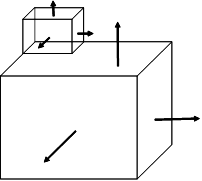
\includegraphics[width=0.9\textwidth, height=0.9\textheight, keepaspectratio=true]{media/image003.png}
\caption{  Example Chart from Standard Output File \protect \label{fig:example-chart-from-standard-output-file}}
\end{figure}


\section{Output does not match EPW values}\label{output-does-not-match-epw-values}

\emph{Why do values in the EPW differ from the output reports of EnergyPlus?}

This is expected. The difference comes from interpolating hourly weather data for subhourly timesteps in EnergyPlus. In an hourly weather file, the temperatures and other state-point readings are the value at the time the reading was taken. For example, in the USA\_IL\_Chicago-OHare\_TMY2.epw file, the outdoor dry bulb value for July 2, hour 1, is 19.4C. This is the temperature at 1:00 am.

If you set Timestep = 1, then EnergyPlus will report 19.4C for 07/02 01:00 and will use that value for the entire one hour timestep.

If Timestep = 4, then 19.4C is used only for the time step which ends at 01:00. The other timesteps use linearly interpolated values between the hourly weather file values. When you report at the ``hourly'' frequency in EnergyPlus, you see the average temperature over the hour. If you report at the ``timestep'' frequency, you will see the values from the weather data file appear at the last timestep of each hour.


\section{Schedules off by 1 hour}\label{schedules-off-by-1-hour}

When active, DaylightSavingTime will shift all scheduled items by one hour. Reporting is always in standard time and uses the same day (scheduled values wrap). In short, the Daylight Saving Time flag uses the schedule value from the \emph{next hour} in the simulation. This can be confusing if your schedules are not symmetric around the midnight hours. Because\ldots{} the new schedule value will show up on the \emph{same day}, not the next day as it might in real life. EnergyPlus does not currently to look ahead/back for next hour schedules (particularly at day boundaries).

More information on Daylight Saving Periods can be seen on the web at: http://www.webexhibits.org/daylightsaving/


\section{Reporting Options}\label{reporting-options}

There are many report variables in EnergyPlus. The ones available for a specific simulation are listed in the report data dictionary (rdd) file. These report variables may be generated automatically if the following is included in the input file.

\begin{lstlisting}

Output:VariableDictionary,
  Regular; !- Key Field
\end{lstlisting}

When the object above is included in an input file, the rdd file is available for review AFTER the simulation has completed. If this object is not included in the input file, the user may still use report variables, but must select them based on the objects included in the simulation. The Input Output Reference document describes all report variables available for each EnergyPlus object.

There are two flavors to output variables: ZONE or HVAC.~ ZONE does not mean that it is a zone variable -- rather, it is produced at the Zone Time Step (the same timestep that you specify in the Timestep object. HVAC type variables, likewise, are produced at the HVAC timestep (which can differ from the zone timestep frequency based on the ConvergenceLimits object).

There are several choices on format with this object. You can specify ``Regular'' as the key field and the rdd will show all report variables along with the variable description as shown below.

\begin{itemize}
\tightlist
\item
  HVAC,Average,Boiler Heating Output Rate {[}W{]}
\item
  HVAC,Sum,Boiler Heating Output Energy {[}J{]}
\item
  HVAC,Average,Boiler Gas Consumption Rate {[}W{]}
\item
  HVAC,Sum,Boiler Gas Consumption {[}J{]}
\item
  HVAC,Average,Boiler Water Inlet Temp {[}C{]}
\item
  HVAC,Average,Boiler Water Outlet Temp {[}C{]}
\item
  HVAC,Average,Boiler Water Mass Flow Rate {[}kg/s{]}
\item
  HVAC,Average,Boiler Parasitic Electric Consumption Rate {[}W{]}
\item
  HVAC,Sum,Boiler Parasitic Electric Consumption {[}J{]}
\item
  HVAC,Average,Boiler Part-Load Ratio {[}{]}
\end{itemize}

As an alternative, the key field ``IDF'' may also be used.

\begin{lstlisting}

Output:VariableDictionary,
  IDF; !- Key Field
\end{lstlisting}

With this option the rdd will format the report variable so that they may be copied directly into the input file using a text editor.

\begin{itemize}
\tightlist
\item
  Output:Variable,*,Boiler Heating Output Rate,hourly; !- HVAC Average {[}W{]}
\item
  Output:Variable,*,Boiler Heating Output Energy,hourly; !- HVAC Sum {[}J{]}
\item
  Output:Variable,*,Boiler Gas Consumption Rate,hourly; !- HVAC Average {[}W{]}
\item
  Output:Variable,*,Boiler Gas Consumption,hourly; !- HVAC Sum {[}J{]}
\item
  Output:Variable,*,Boiler Water Inlet Temp,hourly; !- HVAC Average {[}C{]}
\item
  Output:Variable,*,Boiler Water Outlet Temp,hourly; !- HVAC Average {[}C{]}
\item
  Output:Variable,*,Boiler Water Mass Flow Rate,hourly; !- HVAC Average {[}kg/s{]}
\item
  Output:Variable,*,Boiler Parasitic Electric Consumption Rate,hourly; !- HVAC Average {[}W{]}
\item
  Output:Variable,*,Boiler Parasitic Electric Consumption,hourly; !- HVAC Sum {[}J{]}
\item
  Output:Variable,*,Boiler Part-Load Ratio,hourly; !- HVAC Average {]}
\end{itemize}

A different version of the output variable object is shown below.

\begin{lstlisting}

Output:Variable,
  *, !- Key Value
  Boiler Heating Output Rate, !- Variable Name
  hourly, !- Reporting Frequency
  MyReportVarSchedule; !- Schedule Name

  Schedule:Compact,
  MyReportVarSchedule, !- Name
  On/Off, !- Schedule Type Limits Name
  Through: 1/20, !- Field 1
  For: AllDays, !- Field 2
  Until: 24:00, 0.0, !- Field 4
  Through: 12/31, !- Field 5
  For: AllDays, !- Field 6
  Until: 24:00, 1.0; !- Field 8

  ScheduleTypeLimits,
  On/Off, !- Name
  0:1, !- Range
  DISCRETE; !- Numeric Type
\end{lstlisting}

This allows several options for reporting. First the key value may be an asterisk (*) where all report variables of this type are reported (for all boilers). Or the key value could be specified such that only a single output will be generated. For example if the key value was specified as ``My Boiler'' and a boiler object with the name My Boiler was included in the input, only the Boiler Heating Output Rate for this specific boiler will be in the output file (.csv). The reporting output for all other boilers in the simulation will not be included in the csv file.

The reporting frequency is also another option and may be one of several choices (e.g., Timestep, Hourly, Daily, Monthly, RunPeriod, Environment, Annual or Detailed).

The detailed reporting frequency reports the data for every simulation time step (HVAC variable time steps). This choice is useful for detailed troubleshooting and reporting. The other choices average or sum the data over the selected interval. Timestep refers to the zone Timestep/Number of Timesteps in hour value and reports the data at regular intervals. Using RunPeriod, Environment, or Annual will have the same affect on the reporting frequency and refer to the length of the simulaiton as specified in the RunPeriod object.

\begin{lstlisting}

Timestep,
  4; !- Number of Timesteps per Hour


  RunPeriod,
  1, !- Begin Month
  1, !- Begin Day of Month
  12, !- End Month
  31, !- End Day of Month
  Tuesday, !- Day of Week for Start Day
  Yes, !- Use Weather File Holidays and Special Days
  Yes, !- Use Weather File Daylight Saving Period
  No, !- Apply Weekend Holiday Rule
  Yes, !- Use Weather File Rain Indicators
  Yes; !- Use Weather File Snow Indicator
\end{lstlisting}

A schedule may also be used to turn on or off report variable at selected intervals.

Table reports and meters are also available as reporting options. See the Input Output and Engineering Reference manuals for further details.


\section{Output Variables in IDF Editor}\label{output-variables-in-idf-editor}

You must run the simulation before anything will show in the dropdown menu (rdd/mdd files must be present).


\section{Output Variable Definition}\label{output-variable-definition}

In order to define output variables in your simulation, you must place the following statement in your input file:

\begin{lstlisting}

Output:VariableDictionary,IDF;
\end{lstlisting}

Then you can cut and paste from the rdd file directly into your idf file. You must first run your simulation to create the rdd file. Output variables found in the rdd file are specific to the simulation and are based on the objects used in your input file.

\begin{lstlisting}

Output:Variable,*,System Node Temp,hourly; !- HVAC Average [C]
\end{lstlisting}

To get only information for a single node, change to: Output:Variable,``The Name of the Node'',System Node Temp,hourly; !- HVAC Average {[}C{]}.

Where ``The Name of the Node'' is the specific node name for one or more nodes.


\section{Advanced Output Variable Reporting}\label{advanced-output-variable-reporting}

Files for the following exercise can be found in the ExampleFiles\textbackslash{}AdvancedOutput folder in your installation. A four page instruction sheet is included.

A shortened, bulleted list of steps is shown:

\begin{itemize}
\item
  run the existing input file to generate a list of the report variables available for your simulations.
\item
  add report variables at various time aggregations to the file and run the simulation again.
\item
  create a .RVI file to extract specific data at various time aggregations.
\end{itemize}

Read more about obtaining custom output files (.CSV) using .RVI (Report Variable Input) files from the output in the InputOutputReference.pdf, subject: Using ReadVarsESO.

Simply said, an .RVI is a text file with a list of report variables that you want reported in a .CSV. You can easily develop multiple .RVI files which create different types of .CSV files. For example, separate .CSVs for only the exterior environment data or for only equipment energy consumption. MVI files are the equivalent kind of files for meter only output files (the .mtr files). Both .RVI and .MVI files follow this structure:

\begin{lstlisting}
eplusout.eso   ! name of input eso file
eplusout.csv   ! name of target csv file (or .tab)
\end{lstlisting}

 \ldots{} 0

The first two lines are the default output file .ESO and the default .CSV filename. This is followed by a list of report variables, with the last line containing a 0.

1~~~ Run the ExerciseOutput1.IDF file.

2~~~ Open ExerciseOutput1.RDD and select at least 10 loads-related variables. \emph{Note in ExerciseOutput1.IDF, the object ``Output:VariableDictionary, idf;'' writes the RDD output file as complete objects which can be pasted directly into the IDF file and then edit the reporting frequency.}

Edit ExerciseOutput1.IDF using the text editor, and save as ExerciseOutput1A.IDF. Paste output:variable objects for each of your loads-related variables requesting hourly data. Then copy each object and paste in 4 copies for a total of 5. Then edit the frequency parameter on each, changing ``hourly'' to timestep, daily, monthly, and annual, retaining hourly for one of them. There are already system related output variables with multiple reporting frequencies in the .idf file that you can use as a model. For example, Zone Window Heat Gain and Zone Window Heat Loss, insert these objects in your IDF to get data at each of these time steps:

\begin{itemize}
\item
  Output:Variable, *, Zone Window Heat Gain, timestep;
\item
  Output:Variable, *, Zone Window Heat Gain, hourly;
\item
  Output:Variable, *, Zone Window Heat Gain, daily;
\item
  Output:Variable, *, Zone Window Heat Gain, monthly;
\item
  Output:Variable, *, Zone Window Heat Gain, annual;
\item
  Output:Variable, *, Zone Window Heat Loss, timestep;
\item
  Output:Variable, *, Zone Window Heat Loss, hourly;
\item
  Output:Variable, *, Zone Window Heat Loss, daily;
\item
  Output:Variable, *, Zone Window Heat Loss, monthly;
\item
  Output:Variable, *, Zone Window Heat Loss, annual;
\end{itemize}

\emph{Note that this step may also be done using IDF Editor. When an RDD file is present, the Output:Variable object will have an active drop-down list showing all of the report variable names present in the RDD output file.}

\begin{itemize}
\item
  Run the ExerciseOutput1A.IDF file.
\item
  Using your text editor, open ExerciseOutput1A.idf. Open a new file, and save it as ExerciseOutput1A-LOADS.RVI. Type in the following: 
\end{itemize}

\begin{lstlisting}
eplusout.eso eplusout.csv
\end{lstlisting}

In the .idf file, locate the Output:Variable commands you just added. Copy them, and paste them into the new .RVI file. Delete the duplicates with different reporting frequencies, saving one instance of each variable. Delete everything but the variable name. Add a final line containing only a 0 (zero). For Window Heat Loss and Heat Gain, the .RVI file would look like this:

\begin{lstlisting}
eplusout.eso
eplusout.csv
Zone Window Heat Gain
Zone Window Heat Loss
0
\end{lstlisting}

\begin{itemize}
\item
  Rename file ``ExerciseOutput1-CustomCSV.b\textasciitilde{}t'' to ``ExerciseOutput1¬CustomCSV.bat'' and edit this file in a text editor to make sure the path at the top of the file matches where your version of EnergyPlus is installed. The current path in the file is:
\item
  set post\_proc = C:\textbackslash{}EnergyPlusV6-0-0\textbackslash{}PostProcess\textbackslash{}
\item
  Open a Command Window (Start, Run, Command)
\item
  Change to the directory containing your ExerciseOutput1A.IDF, results files, and your new ExerciseOutput1A-LOADS.RVI. For example:
\item
  CD D:\textbackslash{}EnergyPlus Training\textbackslash{}EnergyPlusExercises ßsubstitute your path here
\end{itemize}

Note: This assumes that the ExerciseOutput1-CustomCSV.bat file is located in the same directory as your IDF and RVI. This is what EP-Launch does for single simulations.

\begin{itemize}
\tightlist
\item
  Type: ExerciseOutput1-CustomCSV ExerciseOutput1A ExerciseOutput1A-LOADS and press Enter. That is,
\end{itemize}

ExerciseOutput1-CustomCSV ExerciseOutput1A ExerciseOutput1A-LOADS

\begin{itemize}
\tightlist
\item
  ExerciseOutput1-CustomCSV reads the ESO output and creates a .CSV for the .RVI for only the variables listed in the .RVI. A .CSV is created for each of the time steps in the output file--timestep, hourly, daily, monthly, or runperiod: inputfilename\_timestep.csv, or for this exercise, ExerciseOutput1A.idf:
\end{itemize}

ExerciseOutput1A\_timestep.csv

ExerciseOutput1A\_hourly.csv

ExerciseOutput1A\_daily.csv

ExerciseOutput1A\_monthly.csv

ExerciseOutput1A\_annual.csv

\emph{If there is no data at the requested time step, that .CSV file will be empty, although that should not occur here.}

\begin{itemize}
\tightlist
\item
  Add report variables to the IDF for energy end-uses. Review .RDD, .MDD and .MTR file for variables to include. Open and save ExerciseOutput1A.idf as ExerciseOutput1B.idf. Create an energy end-use .MVI using the same structure as above but replace eplusout.eso with eplusout.mtr in the first line. Rerun the new IDF and run ExerciseOutput1-CustomCSV again:
\end{itemize}

ExerciseOutput1-CustomCSV ExerciseOutput1B ExerciseOutput1B-ENERGYENDUSE

\begin{itemize}
\tightlist
\item
  Experiment with creating other .RVIs and variables. Example .RVIs for ExerciseOutput1-EquipmentConsumption and ExerciseOutput1-ExternalEnvironment are included.
\end{itemize}


\section{Use of Comma and Point in Numeric Output}\label{use-of-comma-and-point-in-numeric-output}

All EnergyPlus numeric output is written using the U.S. convention of a period or point ``.'' as the decimal separator. No thousands separator is used. For example, the numeric output for ``one thousand two hundred and one half'' would be 1200.5 in output files. The same conventions apply for EnergyPlus input files (idf), Exponent format (1.2005E+03) is also valid on input but is not used in output files.

Commas are used to separate values or fields in EnergyPlus input and output. They should not be used as part of any numeric value, not as a decimal separator and not as a thousands separator. This can cause problems for users in regions of the world which normally use comma as the decimal separator. This is especially important when viewing EnergyPlusvariables (*.csv) and meters (*Meter.csv) output files. Typically csv output files are viewed in a spreadsheet program, such as Excel. ``csv'' stands for ``comma separated values'', so the spreadsheet software needs to recognize comma as a list separator, not a decimal or thousands separator. If the values from a csv file appear to be nonsense when displayed in a spreadsheet program, this may be the source of the problem. Change the decimal separator to be ``.''~ in your system settings or in the spreadsheet program settings.


\chapter{Utilities}\label{utilities}

EnergyPlus comes with a wide variety of pre- and post-processing that are found in the PreProcess and PostProcess folders in the main EnergyPlus install folder.  These utilities have been developed since the initial release of EnergyPlus and can be helpful during the creation of input data for EnergyPlus or interpreting its output.

\chapter{Documentation and Guides}\label{documentation-and-guides}

Note that all of the documentation for EnergyPlus are formatted as PDF documents and fully indexed and searchable. This will save you time while you are waiting for support to answer on some questions or may even help you find the answer you are looking for without needing to contact support.


\chapter{Errors and Warnings}\label{errors-and-warnings}


\section{Max iterations exceeded}\label{max-iterations-exceeded}

\emph{I get the ``Max Iteration'' warning often, in varying quantities. I'd like to understand better what they mean.~}

\emph{1) If these are a concern, at what frequency? (e.g., ``whenever it occurs more than 100? 500? 1000? times in a full year run.'')}

\emph{2) Roughly how much does it affect accuracy of the simulation? (A lot or a little? proportional to the number of occurrences?)}

\emph{3) Any tips about how to avoid it?}

This is a good question, but it is difficult to answer.~ It is something to be concerned about, but in many cases there does not seem to be a way to completely eliminate them and they aren't necessarily a cause for alarm.

\begin{enumerate}
\def\labelenumi{\arabic{enumi})}
\item
  The total count is a difficult measure to use because it varies with number of zones, number and type of air systems, and length of run period.~ A 1,000 might not be a problem for a big model with an annual run, but it could be way too many for a single zone design day run.~ The errors are more common with VAV than CV. The frequency is key though.~ I look at the timing of the errors. If they happen every time step during some period, then it usually means there is something wrong with HVAC.~ If they happen only sometimes, and those times are when things are changing quickly (like recovery from setback), then I don't worry much.
\item
  It depends if the system is succeeding at controlling the zone conditions.~ If the systems are controlling well, and the errors are intermittent, then the results are probably not affected significantly.~ If the systems are not controlling zone conditions, then the errors are probably very significant.~ Check the comfort conditions and zone air temperatures to see.
\item
  When the errors are significant, they usually indicate something is wrong with HVAC input that EnergyPlus isn't able to trap in some other way.~ Possibilities include all sorts of things that can go wrong such as:~ systems connected wrong (node connections usually), sized wrong (mixing hard and auto sizes), controlled wrong (check operation of set point managers by reporting node set point values).
\end{enumerate}


\chapter{Error Messages (Details)}\label{error-messages-details}

Error messages are produced from several parts of EnergyPlus and at several times prior to and during Input Processing (comparing IDF fields/values to IDD requirements); during GetInput for each module (further checking for correct values from the IDF); during Sizing operations; during Warmup operations; and finally during simulation of the environments.

It is easy to separate the Sizing and Warmup errors from the rest. A summary is provided at the end of the simulation:

\begin{lstlisting}
************* EnergyPlus Warmup Error Summary. During Warmup: 0 Warning; 0 Severe Errors.
************* EnergyPlus Sizing Error Summary. During Sizing: 0 Warning; 0 Severe Errors.
************* EnergyPlus Completed Successfully-- 1 Warning; 0 Severe Errors; Elapsed Time = 00hr 00min  6.58sec
\end{lstlisting}


\section{Standard Error Message Format}\label{standard-error-message-format}

Standard error message format changes depending on where the error message is coming from. The standard error message format for GetInput goes something like this:

\textless{}modulename\textgreater{}\textless{}routine name\textgreater{}: \textless{}object name\textgreater{} = \textless{}name field\textgreater{} ``condition''

\textless{}several lines with more information may follow\textgreater{}

The \textless{}modulename\textgreater{}(optional) \textless{}routinename\textgreater{} part is so that people answering support questions can more easily find the code, if necessary and without running the input file through the debugger.

As noted elsewhere, errors come in several flavors with typical user responses required.

In the examples for this section, the severity (Warning/Severe/Fatal) will be left off the message unless necessary for the rest of the example. For example:

\textbf{GetPlantLoopData/GetPlantAvailabilityManager:} AvailabilityManagerAssignmentList = ALWAYS\_ON not found in lists.~ No availability will be used.

Here the routine GetPlantLoopData/GetPlantAvailabilityManager for object AvailabilityManagerAssignmentList with name Always\_On is not found. And then the result is shown.~ (This is a warning level error, by the way).

The development team is working to standardize the error format, as time allows. So, sometimes you will likely see something like:

Check input. Pump nominal power or motor efficiency is set to 0, for pump = HEAT RECOVERY CIRC PUMP

Here, at least you know which pump (Heat Recovery Circ Pump) has the power or motor efficiency of 0.


\section{Example Error Messages for Preprocessors}\label{example-error-messages-for-preprocessors}

All of the preprocessing programs (e.g., EP-Macro, ExpandObjects) produce Output:PreprocessorMessage objects for the errors they detect. Any preprocessor can produce these objects.~ You may need to consult with actual preprocessor program documentation to understand these errors. The output preprocessor messages appear first in the .err file. The format for the messages are: \textless{}objectname\textgreater{} (i.e.~Output:Preprocessormessage) followed by the program name (e.g.~EPMacro) in quotes and then the strings for the message, whether Warning, Severe or Fatal.~ If Fatal, EnergyPlus will fatal out after producing all the error messages.

Here are some examples:

\subsection{Warning}\label{warning-000}

\begin{lstlisting}
Output:PreprocessorMessage = "EPXMLPreProc2" has the following Warning conditions:
   **   ~~~   ** Problem with the width for requested floor area and
   **   ~~~   ** perimeter depth.  Reduced perimeter depth from 4.57
   **   ~~~   ** to 3.656 to accommodate perimeter and core layout
\end{lstlisting}

\subsection{Severe}\label{severe-000}

\begin{lstlisting}
Output:PreprocessorMessage = "EPMacro" has the following Severe conditions:
   **   ~~~   ** at approximately input line number = 200: column = 11
   **   ~~~   ** cannot find/read include file
   **   ~~~   ** symbol = HVAC3ZoneMat-Const.imf
   **   ~~~   ** refer to <file>.epmdet for details.
\end{lstlisting}

Some preprocessor utility programs will give more details than others.~ Here, you see at input file line number 200, about column 11, that the program cannot find (or read) the include file and that there will be more details after the end of EnergyPlus processing in the file with epmdet for extension.

\begin{lstlisting}
Output:PreprocessorMessage = "GroundTempCalc - Slab" has the following Fatal condition:
   **   ~~~   ** No in.epw file found
\end{lstlisting}

This message is coming from the Slab preprocessor program after the ExpandObjects program has processed the input file and triggered the Slab program to be executed. There is no weather file and the Slab program cannot run.

\subsection{Fatal}\label{fatal-000}

Preprocessor condition(s) cause termination.

As you can see from the above Slab message, preprocessor programs may signal a fatal condition but the actual message you see in the .err file is a Severe. You will see the above message if any of the preprocessor conditions signaled a fatal error.


\section{Example Error Messages for the Input Processor}\label{example-error-messages-for-the-input-processor}

The InputProcessor is a part of the EnergyPlus program and scans each input file, matching it against requirements from the Energy+.idd file (Input Data Dictionary). InputProcessor errors all start with IP as their first characters.

\subsection{Warning}\label{warning-001}

\begin{lstlisting}
IP: Note -- Some missing fields have been filled with defaults. See the audit output file for details.
\end{lstlisting}

This message notes that you have some objects where the ``min-fields'' for the object have not been fulfilled and, therefore, the object will be filled with defaults. If you are curious, open the .audit file and search for Warnings.

\subsection{Severe}\label{severe-001}

\begin{lstlisting}
IP: IDF line~345 Did not find "UNTIL: 22:00" in list of Objects
\end{lstlisting}

You may have entered a semi-colon character (;) at the end of one of the lines in a Schedule:Compact input when you meant to enter a comma (,). Note that the approximate line number in your file (345) is given to help you locate it in a text editor. Look in the prior line -- it probably needs to end in a comma.

\begin{lstlisting}
IP: IDF line~xxx Did not find "xxxxxx" in list of Objects
\end{lstlisting}

Same basic description as the previous error message.~ The line number in your file is given to help you locate it.~ Look in the prior line (ignoring any comment lines) -- it probably needs to end with a comma.

\begin{lstlisting}
IP: No items found for Required Object = BUILDING
IP: Required Object = "BUILDING" not found in IDF.
\end{lstlisting}

The Building object is required for all inputs.~ It was not found in this input file.

\begin{lstlisting}
IP: No items found for Required Object = GLOBALGEOMETRYRULES
IP: Required Object = "GLOBALGEOMETRYRULES" not found in IDF.
\end{lstlisting}

The GlobalGeometryRules object is required for all inputs. It was not found in this input file.

\begin{lstlisting}
IP: Possible incorrect IDD File
IDD Version:"IDD\_Version xxx"
Possible Invalid Numerics or other problems
\end{lstlisting}

This message means the program is about to terminate. You look at previous error messages in the .err file to determine the most likely cause(s). The IDD version number is given in case you have an ``x'' version file and you are running it with a ``y'' version IDD (which may or may not work, in general).

\subsection{Fatal}\label{fatal-001}

\begin{lstlisting}
IP: Errors occurred on processing IDF file. Preceding condition(s) cause termination.
\end{lstlisting}

Just the final note before the program terminates. Look at previous error messages in the .err file.


\section{Example Error Messages from Module GetInput routines}\label{example-error-messages-from-module-getinput-routines}

As the simulation starts, each module gets called and gets the values from the input file. These are usually referred to as GetInput routines. They add another error check on the inputs that cannot be fully described by the IDD limits plus they are privy to interactions that their object may have to another object.

\subsection{Warning}\label{warning-002}

\begin{lstlisting}
Site:GroundTemperature:BuildingSurface: Some values fall outside the range of 15-25C.
These values may be inappropriate.  Please consult the Input Output Reference for more details.
\end{lstlisting}

Ground temperatures can have a significant influence on buildings. Values outside the range indicated may give you inaccurate simulation temperatures. Consult the Input Output Reference for more details.

\begin{lstlisting}
GetSurfaceData: CAUTION -- Interzone surfaces are usually in different zones
Surface = WALLMASS, Zone = ZONE1
Surface = iz-WALLMASS, Zone = ZONE1
\end{lstlisting}

Conventionally, interzone surfaces separate two zones. However, some advanced users may create them in the same zone for certain heat transfer efficiencies. This warning message alerts you in case that was not your intention.

\begin{lstlisting}
Weather file location will be used rather than entered Location object.
..Location object = ATLANTA
..Weather File Location = Tampa International Ap FL USA TMY3 WMO# = 722110
..due to location differences, Latitude difference = [5.68] degrees, Longitude difference = [1.89] degrees.
..Time Zone difference = [0.0] hour(s), Elevation difference = [98.10] percent, [309.00] meters.
\end{lstlisting}

You have ``attached'' a weather file that contains different location information than your Site:Location object. The program is warning you of this condition.

\begin{lstlisting}
GetPollutionFactorInput: Requested reporting for Carbon Equivalent Pollution, but insufficient information is entered.
\end{lstlisting}

Both ``FuelFactors'' and ``EnvironmentalImpactFactors'' must be entered or the displayed carbon pollution will all be zero.

You have requested reporting for Carbon Equivalent Pollution (output variables) but you have not entered the required FuelFactor and EnvironmentalImpactFactor objects that are necessary to trigger these outputs properly.

\begin{lstlisting}
BuildingSurface:Detailed = "SURF:xyz", Sun Exposure = "SUNEXPOSED".
 ..This surface is not exposed to External Environment.  Sun exposure has no effect.
\end{lstlisting}

The surface has been entered with SunExposed but it is not an exterior/outdoor surface.

\begin{lstlisting}
GetSurfaceData: InterZone Surface Areas do not match as expected and might not satisfy conservation of energy:
   Area = 1.4E-002 in Surface = 319767, Zone = 2PAV_CONDIC_LOJA_D
   Area = 67.0 in Surface = 6C0708, Zone = 3PAV_CONDIC_TEATRO_G
\end{lstlisting}

Interzone surface areas usually should be matching between the two zones.

\begin{lstlisting}
GetSurfaceData: InterZone Surface Azimuths do not match as expected.
   Azimuth = 270.0, Tilt = 90.0, in Surface = 319767, Zone = 2PAV_CONDIC_LOJA_D
   Azimuth = 180.0, Tilt = 90.0, in Surface = 6C0708, Zone = 3PAV_CONDIC_TEATRO_G
..surface class of base surface = Wall
\end{lstlisting}

Interzone surfaces should be opposite each other -- therefore when Azimuth/Facing do not differ by 180 degrees, a warning is shown. Likewise, Tilt angles should be checked here.

\begin{lstlisting}
GetVertices: Floor is upside down! Tilt angle = [0.0], should be near 180, Surface = "ROOM302-FLOOR", in Zone = "ROOM302".
Automatic fix is attempted.
\end{lstlisting}

\begin{lstlisting}
GetVertices: Roof is upside down! Tilt angle = [180.0], should be near 0, Surface = "ROOM302-CEILING", in Zone = "ROOM302".
Automatic fix is attempted.
\end{lstlisting}

In both of these messages, it has been detected that the outward surface normal for the surfaces is not as expected. With not as expected angles, the sun will not be received on these surfaces (typically), so it is something to correct. The program attempts to fix these -- usually caused by entering the vertices backwards (i.e.~clockwise when should have been counter-clockwise or vice versa).

\begin{lstlisting}
GetInternalHeatGains: Zone = "02AO_FCU04_AN" occupant density is extremely high.
Occupant Density = [14] person/m2.
Occupant Density = [7.000E-002] m2/person. Problems in Temperature Out of Bounds may result.
\end{lstlisting}

The Get Internal Heat Gains routine does some checks as far as Design Level (and maximum schedule * Design Level) and compares to density values. Extremely high gains, especially when no exit for the air (i.e.~infiltration, ventilation) can often result in Temperature Out of Bounds errors (see below in Simulation messages) and these can be fatal.

\begin{lstlisting}
GetVertices: Distance between two vertices < .01, possibly coincident. for Surface = 1%PIANOINTERRATO:UFFICI_WALL_3_0_1, in Zone = 1%PIANOINTERRATO:UFFICI
Vertex [2] = (-53.99,5.86,0.50)
Vertex [1] = (-53.99,5.86,0.51)
Dropping Vertex [2].
\end{lstlisting}

The distance between two vertices is very small (.01 meter \textasciitilde{} .4 inches). This distance is too small for shading calculations and the vertex is dropped.

\begin{lstlisting}
CheckConvexity: Surface = "ZN001:ROOF001" is non-convex.
\end{lstlisting}

Shown when DisplayExtraWarnings is on and a surface is not a convex shape. By itself, this is only a warning but see the severe in the next section when it has impact on the calculations.

\subsection{Severe}\label{severe-002}

\begin{lstlisting}
GetSurfaceData: Some Outward Facing angles of subsurfaces differ significantly from base surface.
...use Output:Diagnostics,DisplayExtraWarnings; to show more details on individual surfaces.
\end{lstlisting}

\begin{lstlisting}
GetSurfaceData: Outward facing angle [95.5] of subsurface = "WL2-1" significantly different than
..facing angle [275.5] of base surface = WEST WALL 2 Tilt = 90.0
..surface class of base surface = Wall
\end{lstlisting}

These are two versions of the same message.~ The first is shown when DisplayExtraWarnings is not activated. The second is shown for details on each subsurface that has the error.~ The error is usually that the subsurface vertices have been entered in opposite order (i.e.~clockwise vs counter-clockwise) from the base surface.

\begin{lstlisting}
This building has no thermal mass which can cause an unstable solution.
Use Material object for all opaque material definitions except very light insulation layers.
\end{lstlisting}

You have probably defined all the surfaces in this building with resistive only constructions (i.e.~object Material:NoMass). An unstable solution can result (including crashes).

\begin{lstlisting}
GetVertices: Distance between two vertices < .01, possibly coincident. for Surface = 1%PIANOINTERRATO:UFFICI_WALL_3_0_1, in Zone = 1%PIANOINTERRATO:UFFICI
Vertex [3] = (-44.82,-12.14,0.51)
Vertex [2] = (-44.82,-12.14,0.50)
Cannot Drop Vertex [3].
Number of Surface Sides at minimum.
\end{lstlisting}

The distance between two vertices is very small (.01 meter \textasciitilde{} .4 inches). This distance is too small for shading calculations but the vertex cannot be dropped as that would bring the surface to less than 3 sides. This surface is degenerate and should be removed from your input file.

\begin{lstlisting}
DetermineShadowingCombinations: Surface = "0%VESPAIO:ZONA1\_ROOF\_1\_6\_0" is a receiving surface and is non-convex.
...Shadowing values may be inaccurate. Check .shd report file for more surface shading details
\end{lstlisting}

Receiving surfaces which are not convex shapes will not be calculated correctly with the shadowing routines. You should view the results carefully.

\subsection{Fatal}\label{fatal-002}

Severes in this realm usually lead to Fatals. Preceding conditions lead to termination.


\section{Example Error Messages during Sizing and Simulation}\label{example-error-messages-during-sizing-and-simulation}

\subsection{Warning}\label{warning}

\begin{lstlisting}
Calculated design cooling load for zone = B1AE_FCU02_AN is zero.
Check Sizing:Zone and ZoneControl:Thermostat inputs.
\end{lstlisting}

\begin{lstlisting}
Calculated design heating load for zone = B1AE\_FCU02\_AN is zero.
Check Sizing:Zone and ZoneControl:Thermostat inputs.
\end{lstlisting}

Two flavors of the same message showing up during Sizing. Read about Day Types in the Sizing:* objects.~ Schedules may affect how the program looks at loads during sizing. Another suggestion is:

Plot the zone temperature and check against the zone thermostat set point temperature.

\begin{lstlisting}
Output:Variable,*,Zone/Sys Air Temperature at Thermostat,timestep;
Output:Variable,*,Zone/Sys Thermostat Heating Setpoint,timestep;
\end{lstlisting}

If the zone temperature never falls below the thermostat set point temperature then there really is no load and lighting, equipment, occupancy, etc inputs/schedules need to be checked. Usually these types of load will be turned off for the design days in winter to correctly size the heating system. If the zone temperature does fall below the zone thermostat temperature, then the zone sizing objects probably have bad inputs.

\subsection{Severe}\label{severe}

\begin{lstlisting}
Temperature (high) out of bounds (206.82] for zone = "ZONE 1", for surface = "SOUTH WALL"
During Warmup & Sizing, Environment = ALEXANDRIA ESLER REGIONAL AP ANN HTG 99.6% CONDNS DB, at Simulation time = 12/21 01:00 - 01:04
Zone = "ZONE 1", Diagnostic Details:
...Internal Heat Gain [155.557] W/m2
...Infiltration/Ventilation [3.500E-002] m3/s
...Mixing/Cross Mixing [0.000] m3/s
...Zone is part of HVAC controlled system.
\end{lstlisting}

This error may be related to one of the warnings during get input routines on the Design Level of some heat gains at the zone level. Also to be noted here is the amount of Infiltration/Ventilation being introduced at the zone level. This diagnostics detail is produced once for each zone where the error occurs.

\subsection{Fatal}\label{fatal}

\begin{lstlisting}
EnergyPlus has exited due to the reason stated above
...Summary of Errors that led to program termination:
..... Reference severe error count = 11
..... Last severe error = Temperature (high) out of bounds (210.11] for zone = "ZONE 1", for surface = "ROOF1"
\end{lstlisting}

Typical fatal condition. A small summary of the number of severe errors that were produced along with the last severe error.


\section{Recurring Errors}\label{recurring-errors}

The recurring error category is employed during the actual simulation periods. Usually, a heading message will appear:

\begin{lstlisting}
   ** Warning ** Coil:Cooling:DX:SingleSpeed "DXCOOLINGCOIL_SOUTHZONE_2NDFLOOR" - Full load outlet air dry-bulb temperature < 2C. This indicates the possibility of coil frost/freeze. Outlet temperature = -4.60 C.
   **   ~~~   **  ...Occurrence info = Washington Dc Dulles IntL Ar VA USA TMY3 WMO# = 724030, 01/02 06:01 - 06:02
   **   ~~~   ** ... Possible reasons for low outlet air dry-bulb temperatures are: This DX coil
   **   ~~~   **    1) may have a low inlet air dry-bulb temperature. Inlet air temperature = 9.778 C.
   **   ~~~   **    2) may have a low air flow rate per watt of cooling capacity. Check inputs.
   **   ~~~   **    3) is used as part of a HX assisted cooling coil which uses a high sensible effectiveness. Check inputs.
\end{lstlisting}

This message contains quite a bit of information: the basic object and name of the object, the context of the error, the time of the error as well as some reasons why this might have occurred.

At the end of the simulation, the summary appears:

\begin{lstlisting}
   *************  ** Warning ** Coil:Cooling:DX:SingleSpeed "DXCOOLINGCOIL_SOUTHZONE_2NDFLOOR" - Full load outlet temperature indicates a possibility of frost/freeze error continues. Outlet air temperature statistics follow:
   *************  **   ~~~   **   This error occurred 1240 total times;
   *************  **   ~~~   **   during Warmup 0 times;
   *************  **   ~~~   **   during Sizing 0 times.
   *************  **   ~~~   **   Max = 1.995912  Min = -4.60024
\end{lstlisting}

Here you see a summary of how many times the error occurred (1240) as well as how many times during Warmup (0) and how many times during Sizing (0). Plus a minimum (-4.6) and maximum (1.99) for the terms of the message.


\section{Summaries at End of Simulation}\label{summaries-at-end-of-simulation}

Some classes of warnings produce more information at the end of the simulation. For example,

\begin{lstlisting}
Loads Initialization did not Converge (CheckWarmupConvergence) after 25 warmup days.
Environment = SAN_FRANCISCO ANN CLG 1% CONDNS DB = >MWB
Max Temp Comparison = 9.15E-002 vs Temperature Convergence Tolerance = 4.00E-003 - Fail Convergence
Min Temp Comparison = 1.75E-003 vs Temperature Convergence Tolerance = 4.00E-003 - Pass Convergence
Max Cool Load Comparison = 2.9010E-002 vs Loads Convergence Tolerance = 4.00E-002 - Pass Convergence
Then, at the end of the simulation, you will see:
******** The following error categories occurred.  Consider correcting or noting.
******** Loads Initialization did not Converge
******** ..1) very high thermal mass such as very thick concrete (solution: increase max number of warmup
******** ..   days in the BUILDING object);
******** ..2) moderate mass and inadequate space conditioning such that the building keeps getting warmer
******** ..   and warmer on successive days (solution: add HVAC, check building thermal properties,
******** ..   check if infiltration is included, make sure HVAC properly controlled);
******** ..3) a soil layer modeled below the concrete slab - (solution remove this layer and read about
******** ..   ground temperatures in the Auxiliary Programs document).
******** ..4) unreasonable (too small) limits in the BUILDING object for temperature (.4 default) or
******** ..   loads tolerances (.04 default)
\end{lstlisting}


\section{Psychrometric Errors}\label{psychrometric-errors}

EnergyPlus has built-in psychrometric routines that perform various calculations for the simulation modules. They typically fall into the recurring error category but may warrant some view:

\begin{lstlisting}
   ** Warning ** Calculated Relative Humidity out of range (PsyRhFnTdbWPb)
\end{lstlisting}

\begin{lstlisting}
   **   ~~~   **  Routine = NodeReportingCalc:NODE_1, Environment = CHICAGO_IL_USA ANNUAL COOLING 1% DESIGN CONDITIONS DB/MCWB, at Simulation time = 07/21 00:00 - 00:10
\end{lstlisting}

\begin{lstlisting}
   **   ~~~   **  Dry-Bulb = 13.00 Humidity Ratio = 1.000E-002 Calculated Relative Humidity [%] = 104.65
\end{lstlisting}

\begin{lstlisting}
   **   ~~~   ** Relative Humidity being reset to 100.0%
\end{lstlisting}

This warning notes that the calculated relative humidity is out of rage (routine name: PsyRhFnTdbWPb). It happened during routine NodeReportingCalc for NODE\_1 at the environment ``CHICAGO\_IL\_USA ANNUAL COOLING 1\% DESIGN CONDITIONS DB/MCWB'' during the time interval 00:00 -- 00:10 on July 21. The dry bulb temperature was 13 C, the humidity ratio was .001 for a calculated relative humidity of 104.65\%. It is reset to 100\%.

Then, at the end of the run, you will see a summary of how many times that occur and the min/max extent:

\begin{lstlisting}
   *************  ** Warning ** Calculated Relative Humidity out of range (PsyRhFnTdbWPb)
\end{lstlisting}

\begin{lstlisting}
   *************  **   ~~~   **   This error occurred 645 total times;
\end{lstlisting}

\begin{lstlisting}
   *************  **   ~~~   **   during Warmup 0 times;
\end{lstlisting}

\begin{lstlisting}
   *************  **   ~~~   **   during Sizing 0 times.
\end{lstlisting}

\begin{lstlisting}
   *************  **   ~~~   **   Max = 104.652877 %  Min = 104.652877 %
\end{lstlisting}


\section{Error Summary}\label{error-summary}

This section has provided a flavor of the breadth of messages coming out of EnergyPlus for various conditions. They are consolidated into one file (eplusout.err) for the most part though some may have more contexts given in other files. (eplusout.audit may illustrate exact places in the IDF where warnings or errors occur -- as noted during Input Processing.)

The error section in this document will continue to grow as time allows. Suggestions are always welcome.


\chapter{Validation and Testing}\label{validation-and-testing}

An important ongoing part of EnergyPlus development is testing using industry standard methods as major builds are completed. The goal is to make EnergyPlus as bug-free as possible. Three major types of tests are currently conducted:

\begin{itemize}
\item
  Analytical tests:
\item
  HVAC tests, based on ASHRAE Research Project 865
\item
  Building fabric tests, based on ASHRAE Research Project 1052
\item
  Comparative tests:
\item
  ANSI/ASHRAE Standard 140-2007
\item
  International Energy Agency Solar Heating and Cooling Programme (IEA SHC) BESTest (Building Energy Simulation Test) methods not yet in Standard 140
\item
  EnergyPlus HVAC Component Comparative tests
\item
  EnergyPlus Global Heat Balance tests
\item
  Release and executable tests
\end{itemize}

For detailed reports, please use the following link:

http://apps1.eere.energy.gov/buildings/energyplus/energyplus\_testing.cfm


\chapter{Platforms and Run-Time}\label{platforms-and-run-time}

EnergyPlus is available for the Windows, Macintosh, and Linux Platforms. It may not be available for all flavors of those platforms. Usually, the newer versions of those platforms will be the ones most supported with some older versions as well.


\section{Reduce EnergyPlus Run Time}\label{reduce-energyplus-run-time}

\emph{What affects EnergyPlus Run-Time?}

Compared with creating energy models either by hand coding the IDF file or by using GUI tools or a combination of both, EnergyPlus run time is normally a small fraction of the total time needed to complete an energy modeling job. Therefore it is very important to build a clean and concise EnergyPlus model up front. Techniques of simplifying large and complex building and systems should be used during the creation of energy models, especially during the early design process when detailed zoning and other information is not available. Producing lots of hourly or sub-hourly reports from EnergyPlus runs can take significant amount of time. Modelers should only request time step reports when necessary. On the other hand, producing summary reports and typical monthly reports take relatively small amount of run time. These reports are valuable references for troubleshooting and model fine tuning.

With powerful personal computers get more and more affordable, EnergyPlus modelers should choose to use current available PCs with 3 or more GHZ clock speed and 3 or more GB of RAM and multiple core processors. EP-Launch will now automatically launch multiple runs on multiple processors (group runs).

For modelers, most time is spent on troubleshooting and fine tuning energy models. During the early modeling process, it is recommended to keep the model as simple as possible and make quick runs to identify problems. Then modify the IDF file to fix problems and re-run the model. This is an iterative process until satisfactory solutions are found. The simulation process can be split into three phases: the diagnostic runs, the preliminary runs, and the final runs. The three phases would use different simulation settings. The diagnostic runs would use a set of simulation settings to speed up the runs with simulation accuracy being set as the second priority. The diagnostic runs will help catch most model problems by running simulations on summer and winter design days. The preliminary runs use a tighter set of simulation settings in order to catch problems missed in the diagnostic runs, and provide better results for quality assurance purpose. The final runs use the EnergyPlus recommended set of simulation settings in order to achieve better accuracy for simulation results ready for review and reporting.

Specifically, recommendations (and particularly recommended for large buildings with large numbers of surfaces and shading surfaces):

% table 5
\begin{longtable}[c]{p{1.5in}p{4.5in}}
\caption{Recommended Reduce Time Settings for Early Diagnostic runs \label{table:recommended-reduce-time-settings-for-early}} \tabularnewline
\toprule 
Object & Recommenheh Early Diagnostic Setting \tabularnewline
\midrule
\endfirsthead

\caption[]{Recommended Reduce Time Settings for Early Diagnostic runs} \tabularnewline
\toprule 
Object & Recommenheh Early Diagnostic Setting \tabularnewline
\midrule
\endhead

Building & MinimalShadowing (Solar Distribution field) \tabularnewline
ShadowCalculation & 200 (Maximum Figures in Shadow Overlap Calculations field) \tabularnewline
SizingPeriod:DesignDays & Only perform design day or limited run period runs until you have the model set. \tabularnewline
\bottomrule
\end{longtable}

You might want to read the report on EnergyPlus run time at http://repositories.cdlib.org/lbnl/LBNL-1311E/

Remember, too, that EnergyPlus is, by design, a multiple timestep per hour simulation. Comparing its run-time to programs that are only hourly has potential for comparing apples and grapes. In addition, EnergyPlus is a simultaneous solution of the building loads, HVAC system and plant equipment simulation with possible multiple iterations to reach balance.


\section{Run EnergyPlus in Parallel}\label{run-energyplus-in-parallel}

EnergyPlus is a multi-thread application but is not optimized for parallel runs on multi-core machines. However, multiple parametric runs can be launched in parallel if these runs are independent. One way to do it is to create multiple folders and copy files EnergyPlus.exe, Energy+.idd, DElight2.dll, libexpat.dll, bcvtb.dll, EPMacro.exe (if macros are used), ExpandObjects.exe (if HVACTemplate or Compact HVAC objects are used) from the original EnergyPlus installed folder. Inside each folder, copy IDF file as in.idf and EPW file as in.epw, then run EnergyPlus.exe from each folder. This is better handled with a batch file. If the Energy+.ini file exists in one of the created folders, make sure it is empty or points to the current EnergyPlus folder.

EP-Launch now does this automatically for Group or Parametric-Preprocessor runs.

The benefit of run time savings depends on computer configurations including number of CPUs, CPU clock speed, amount of RAM and cache, and hard drive speed. To be time efficient, the number of parallel EnergyPlus runs should not be more than the number of CPUs on a computer. The EnergyPlus utility program EP-Launch is being modified to add the parallel capability for group simulations. The long term goal is to run EnergyPlus in parallel on multi-core computers even for a single EnergyPlus run without degradation to accuracy.


\section{Running EnergyPlus on Windows Vista and/or Windows 7}\label{running-energyplus-on-windows-vista-andor-windows-7}

For all operating systems, make sure that you have read and write access to files in the main EnergyPlus folder (by default EnergyPlus is installed in C:\textbackslash{}EnergyPlus\textless{}version\textgreater{}). If you do not have this kind of access some very peculiar messages may appear when you try to run simulations.

EnergyPlus has no problems running on Vista or Windows 7 computers if it is run directly by executing the EnergyPlus.exe file assuming you have prepared the in.idf and in.epw files at the same folder. There were some issues running earlier versions of EP-Launch, but most have been fixed for the latest version of EP-Launch. If EnergyPlus was installed at a user folder like C:\textbackslash{} EnergyPlusV3-0-0, there should be no problems running EP-Launch. If EnergyPlus was installed at a windows system folder like `C:\textbackslash{}Program files\textbackslash{} EnergyPlusV3-0-0', you have to run EP-Launch every time with administrator rights by right clicking the EP-Launch.exe file and choose `Run as Administrator'. Another way is to create a shortcut to EPLaunch and change settings appropriately.


\end{document}
